\documentclass[11pt,a4paper]{article}

\usepackage[utf8]{inputenc}
\usepackage[T1]{fontenc}
\usepackage{lmodern}
\usepackage{microtype}
\usepackage[margin=1.85cm]{geometry}
\usepackage{amsmath,amssymb,amsfonts}
\usepackage{booktabs}
\usepackage{array}
\usepackage{graphicx}
\usepackage{float}
\usepackage[table]{xcolor}
\usepackage{colortbl}
\usepackage[round,authoryear]{natbib}
\usepackage[colorlinks=true,linkcolor=blue!60!black,citecolor=blue!60!black,urlcolor=blue!60!black]{hyperref}
\usepackage{caption}
\captionsetup{font=small,labelfont=bf}

\definecolor{tabhead}{HTML}{D6E4F0}
\definecolor{rowodd}{HTML}{FFFFFF}
\definecolor{roweven}{HTML}{F3F6FA}
\definecolor{colodd}{HTML}{F0F5FA}
\definecolor{coleven}{HTML}{E3ECF5}
\definecolor{rulecol}{HTML}{B8C8D8}

\newcommand{\co}{\cellcolor{colodd}}
\newcommand{\ce}{\cellcolor{coleven}}

\setlength{\parskip}{0.42em}
\setlength{\parindent}{0pt}
\setlength{\tabcolsep}{6.5pt}
\renewcommand{\arraystretch}{1.24}
\arrayrulecolor{rulecol}
\setlength{\arrayrulewidth}{0.55pt}

\title{\textbf{Does Increasing Government Spending on Tertiary Education Improve the Future Tax Take? A Bayesian Causal Inference Analysis}}

\author{
  \textbf{Andrew C. Parnell}\\[0.3em]
  \small School of Mathematics and Statistics, University College Dublin\\
  \small \texttt{andrew.parnell1@ucd.ie}
}

\date{6 November 2026}

\begin{document}

\maketitle

\begin{abstract}
\noindent When a national government increases public spending on tertiary (university) education, does that investment strengthen the country's future tax take once general macroeconomic growth is separated out? Answering this in cross-country panels is hard because faster-growing economies naturally collect more taxes, international indicators divide per-student spending by gross domestic product (GDP) per person and student headcount, and university cohorts take years to enter peak tax brackets. I construct a harmonised panel across 217 sovereign countries from 1985 to 2024 (372 five-year waves across 121 countries at $+5$ years; 283 across 112 countries at $+10$ years) and estimate Multivariate and Longitudinal Bayesian Causal Forests, separating baseline conditions from mediating macroeconomic changes (forward GDP growth, enrolment expansion, inequality, and life expectancy). Above-median per-student tertiary funding shifts revenue composition toward direct income, profit, and capital gains taxation by $+1.24$ percentage points (pp; 95\% CI $[+0.24, +2.40]$, $P = 0.99$, where $P$ is the posterior probability of an effect greater than zero given the data) after 5 years and $+1.48$ pp (95\% CI $[-0.11, +3.03]$, $P = 0.97$) after 10 years, whilst overall non-resource tax revenue changes by $+0.45$ pp of GDP (95\% CI $[-0.35, +1.24]$, $P = 0.86$) and their product, direct income tax revenue, rises by $+0.34$ pp of GDP (95\% CI $[-0.06, +0.76]$, $P = 0.95$) at $+10$ years. Within-country per-student expansions ($\ge +2.5$ pp) raise 10-year direct income taxes by $+0.81$ pp of GDP (95\% CI $[+0.29, +1.33]$, $P = 1.00$), real PPP dollars per student raise 10-year non-resource tax revenue by $+0.94$ pp of GDP (95\% CI $[+0.09, +1.88]$, $P = 0.99$), and longitudinal trajectories ($N = 282$) show 10-year gains of $+1.94$ pp on direct income tax share (95\% CI $[+0.76, +3.22]$, $P = 1.00$) and $+0.41$ pp of GDP on direct income taxes (95\% CI $[+0.09, +0.71]$, $P = 1.00$).

\vspace{0.5em}
\noindent \textbf{Keywords:} Bayesian Causal Forests; tertiary education spending; fiscal capacity; direct income taxation; causal mediation; longitudinal panel data.
\end{abstract}

\section{Introduction}
\label{sec:intro}

Public debates over higher education finance frequently centre on a simple, practical question: is government spending on tertiary (university) education a net drain on the public purse, or is it a productive investment that expands a country's future tax base? At the individual level, decades of labour economics research have shown that university graduates earn higher wages, experience lower unemployment, and work in more formalised firms than non-graduates \citep{carneiro2011estimating, zimmerman2014returns, psacharopoulos2018returns, deming2022four}. Welfare analyses of public expenditure in the United States also suggest that college spending and financial aid policies pay back a large fraction of their upfront budgetary cost when long-term income tax receipts are counted \citep{trostel2010fiscal, hendren2020unified, chakrabarti2020state}. In principle, as university-educated cohorts enter the labour market and raise firm productivity \citep{moretti2004estimating, valero2019economic}, those private wage gains and corporate spillovers should show up at the national level as stronger income, payroll, and corporate profit tax receipts.

Yet working out whether, and over what time horizon, national government spending on tertiary education actually improves a country's tax take is surprisingly tricky. Cross-country fiscal studies run into three main obstacles:

\begin{enumerate}
  \item \textbf{Separating Direct Fiscal Returns from General Economic Growth:} If a country's tax take rises over the decade following an increase in university funding, is that because universities specifically strengthened the formal tax base, or simply because the whole economy grew richer? Worse still, if an analyst constructs a national ``tax take per person'' variable by multiplying the tax-to-GDP ratio by GDP per person, any positive effect of education on GDP automatically inflates the tax outcome by mathematical identity. Isolating the genuine fiscal dividend requires modelling pure tax shares and tax-to-GDP ratios whilst separating starting economic conditions from post-treatment mediating macroeconomic growth \citep{imai2010general, acharya2016explaining, vanderweele2016mediation}.
  \item \textbf{The UNESCO Denominator Trap:} The most widely used international indicator of tertiary funding intensity, compiled by the UNESCO Institute for Statistics and the World Bank, measures public expenditure per tertiary student as a percentage of GDP per person. Because this composite ratio places both student headcount and GDP per person in the denominator, a low-income country with a tiny, elite university sector (such as Malawi or Uganda in the 1990s, enrolling fewer than 2\% of young adults) can appear to spend 150\% of GDP per person per student, whereas a high-income country enrolling 60\% of its young adults (such as Denmark or South Korea) appears to spend 27\%, even though the high-income country spends nearly three times as many real dollars per student. I return to this running example throughout the paper.
  \item \textbf{Maturation Lags and Tax Structure Specificity:} University investments take time to mature. A funding increase in wave $t$ immediately pays formal university salaries and supports student cohorts who take three to five years to graduate and another five years to reach peak tax-paying brackets. Furthermore, public finance theory tells us that as economies accumulate skilled workers and formal employers, they shift away from indirect consumption and customs taxes toward direct personal income and corporate profit taxes \citep{gordon2009tax, besley2014pillars, kleven2016why, jensen2022employment}. Looking only at a single aggregate tax number hides this compositional shift.
\end{enumerate}

\begin{figure}[t!]
  \centering
  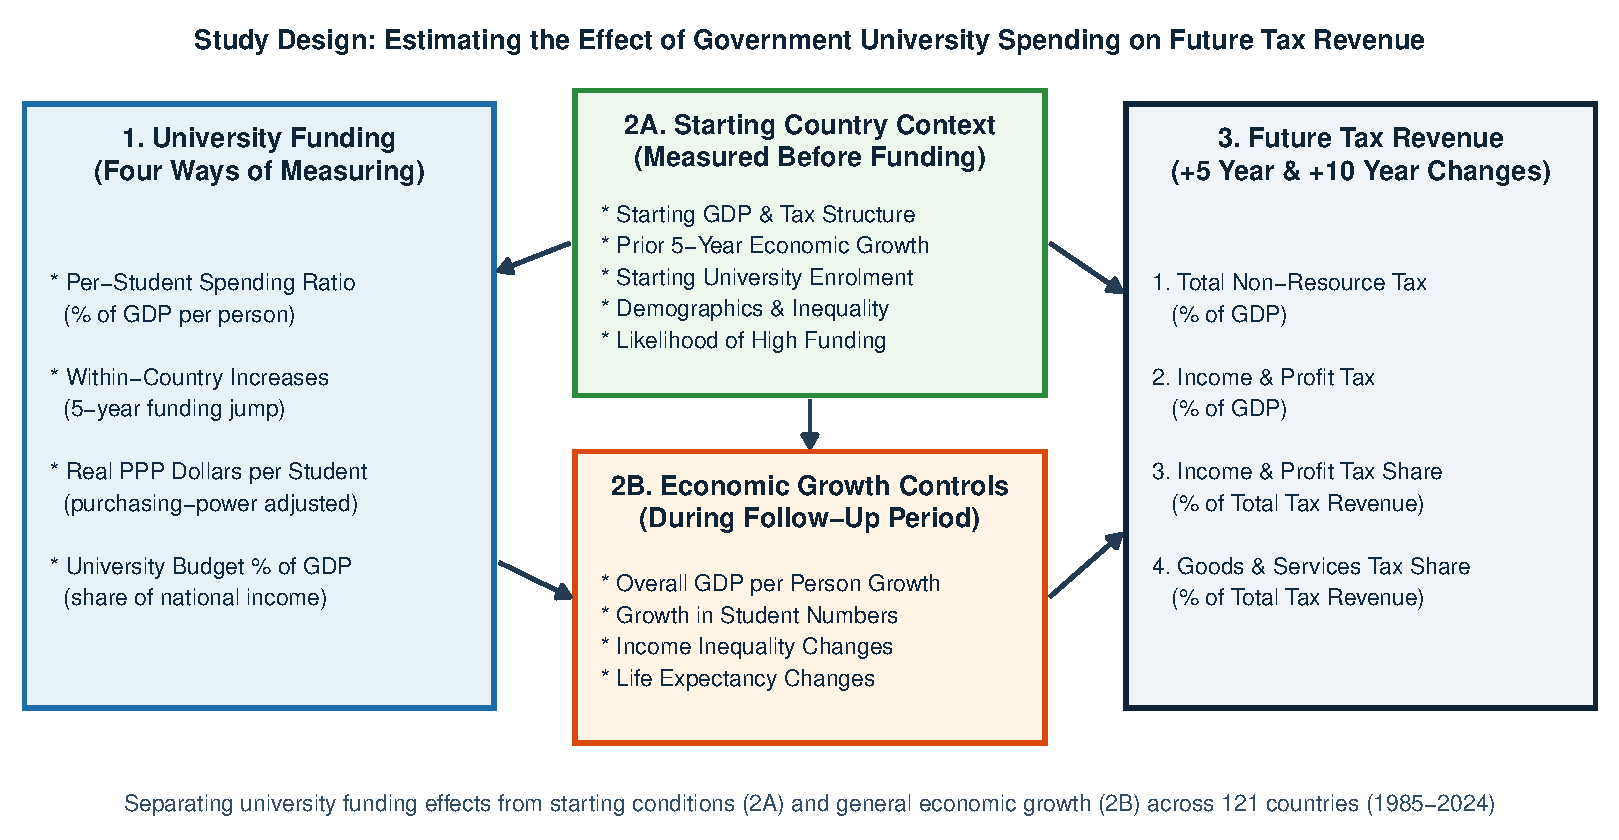
\includegraphics[width=\textwidth]{../outputs/figures/fig1_structural_schematic.pdf}
  \caption{Study design showing how I compare four observed measures of government tertiary education spending, separate baseline country context (Pathway 2A) from mediating macroeconomic changes (Pathway 2B), and track four disaggregated tax outcomes over $+5$ and $+10$ years.}
  \label{fig:schematic}
\end{figure}

Figure~\ref{fig:schematic} shows how I set up this study to tackle all three obstacles:

\begin{itemize}
  \item \textbf{Four Disaggregated Tax Outcomes Spanning Level and Composition:} Rather than multiplying tax ratios by GDP per person, I model four percentage-point (pp) fiscal outcomes jointly: (1) overall domestic non-resource tax revenue as a share of GDP ($\Delta \text{Tax/GDP}$), (2) direct income, profit, and capital gains tax revenue as a share of GDP ($\Delta \text{IncomeTax/GDP}$), (3) direct income and profit taxes as a share of total revenue ($\Delta \text{IncomeTax/Rev}$), and (4) indirect goods and services (consumption and value-added) taxes as a share of total revenue ($\Delta \text{GoodsTax/Rev}$). As I explain in Section~\ref{sec:data}, these four outcomes capture two independent structural dimensions (the aggregate tax-to-GDP level in Outcome 1 and the revenue-share composition between direct and indirect taxes in Outcomes 3 and 4), whilst Outcome 2 represents the policy-relevant product of the two.
  \item \textbf{Unbundling the Tertiary Spending Denominators:} Instead of relying on a single composite ratio, I compare four strictly observed measures of tertiary funding side by side (with zero proxy imputation): the per-student tertiary spending ratio (\% of GDP per person), observed within-country per-student tertiary funding expansions ($\ge +2.5$ pp over a five-year wave), real 2021 purchasing-power-parity (PPP) dollars per tertiary student (removing GDP from the denominator), and the public tertiary budget as a percentage of GDP (removing student headcount from the denominator).
  \item \textbf{Isolating the Mediator-Removed Direct Effect:} Using Multivariate Bayesian Causal Forests \citep{hahn2020bayesian, mcjames2024mvbcf} and a Longitudinal Bayesian Causal Forest \citep{mcjames2024lbcf}, I compare a \textbf{Total Fiscal Effect Model (\texttt{M1})} (conditioning strictly on pre-treatment baseline covariates including lagged economic growth) against a \textbf{Mediator-Removed Direct Fiscal Effect Model (\texttt{M2})}, which additionally removes the mediating pathways of forward GDP per person growth, tertiary enrolment expansion, income inequality changes, and life expectancy changes over the follow-up window. I also check these direct effect estimates using Two-Stage Sequential G-Estimation \citep{acharya2016explaining}.
\end{itemize}

Throughout the remainder of this paper, I use \textbf{pp} to denote percentage points, \textbf{CI} to mean a Bayesian posterior \textbf{credible interval} (unless explicitly flagged as a frequentist confidence interval for linear benchmarks in Section~\ref{sec:benchmarks}), and \textbf{$P = P(\tau > 0 \mid \text{data})$} to mean the posterior probability that the causal treatment effect $\tau$ is strictly greater than zero given the observed data (rounded to two decimal places in accordance with the Monte Carlo standard errors reported in Appendix~\ref{app:diagnostics}).

\paragraph{Paper Structure and Contributions.}
To my knowledge, this is the first global causal inference study to jointly model overall non-resource tax revenue, direct income and profit taxation, and indirect consumption taxation using Multivariate and Three-Wave Longitudinal Bayesian Causal Forests whilst separating the mediator-removed direct fiscal effect from general economic growth and unbundling the UNESCO per-student spending ratio across 121 countries. The paper is structured as follows. Section~\ref{sec:lit} reviews the relevant public finance, higher education, and Bayesian causal forest literatures. Section~\ref{sec:data} describes the 40-year global panel and illustrates the UNESCO denominator trap. Section~\ref{sec:methods} introduces the Multivariate and Longitudinal Bayesian Causal Forest models in plain language (with full mathematical and algorithmic details in Appendix~\ref{app:math}). Section~\ref{sec:results} presents the empirical results, method benchmarks, and robustness checks. Section~\ref{sec:discussion} discusses cohort maturation mechanisms, names the main limitations of my approach, and suggests avenues for future work.

\section{Literature Review and Conceptual Framework}
\label{sec:lit}

In this section I briefly review three strands of research that have largely developed in parallel: the political economy of tax structure modernisation, the economics of per-student university resources, and Bayesian tree ensembles for causal mediation analysis. Those interested in more detailed surveys of each field may refer to \citet{besley2014pillars}, \citet{deming2022four}, and \citet{hill2020bayesian}.

\subsection{Fiscal Capacity, Formal Employment, and Tax Structure Modernisation}

A classic puzzle in public finance is why rich countries collect 30\% to 45\% of GDP in tax revenue (mostly through direct personal income taxes, social contributions, and corporate profit taxes), whereas low- and middle-income countries often collect less than 15\% of GDP and rely heavily on indirect consumption taxes and trade duties \citep{gordon2009tax, besley2009origins, besley2014pillars}. Early macro-fiscal studies emphasised political institutions, property rights, and state capacity \citep{besley2009origins, kaufmann2011worldwide}, alongside better cross-national accounting to separate domestic taxes from volatile natural resource royalties \citep{prichard2016reassessing, ictd2023grdv}.

More recently, empirical public finance has focussed on the microeconomic mechanics of tax enforcement, paper trails, and formal employment \citep{kleven2016why, keen2017optimal, pomeranz2019taking}. \citet{kleven2016why} show that modern governments can enforce high direct tax compliance at low audit cost because large, formal firms act as third-party tax collectors: complex businesses need internal accounting records shared amongst managers and skilled staff, which makes colluding to hide wages and profits very difficult. Building on this idea, \citet{jensen2022employment} assembles household micro-data across nearly 100 countries and shows that the shift from informal self-employment into salaried employee jobs is the main driver of income tax growth as countries develop. Field experiments and administrative studies confirm that electronic tax filing and third-party reporting curb evasion when paired with capable firms and literate taxpayers \citep{pomeranz2019taking, okunogbe2022technology}, whilst broader direct taxation can also encourage citizens to hold governments accountable \citep{weigel2020participation}. By contrast, in developing economies with large informal sectors, consumption taxes such as value-added tax (VAT) remain the fallback option because formal retail chains only gradually replace informal street vendors as incomes rise \citep{bachas2024informality}.

I think this fiscal-capacity literature points to a direct link between university funding and the tax base that goes well beyond headline GDP growth. Universities are themselves large formal employers whose staff pay income tax through automatic payroll withholding, and they train the professional, managerial, scientific, and accounting workers needed by formal firms \citep{kleven2016why, valero2019economic}, moving workers into salaried jobs above national income tax exemption thresholds \citep{jensen2022employment}. If this mechanism operates at the national level, higher public spending per university student should specifically boost \textbf{direct income, profit, and capital gains taxation} as a share of total revenue and as a share of GDP, whilst reducing relative reliance on indirect goods and services taxes.

\subsection{Returns to Tertiary Education, Per-Student Resources, and Fiscal Externalities}

A large microeconometric literature finds strong private wage returns to university education across both rich and poor countries \citep{carneiro2011estimating, zimmerman2014returns, psacharopoulos2018returns, chetty2020income, mountjoy2022community}. Reviewing this evidence, \citet{deming2022four} notes that human capital explains at least one-third of within-country wage variation and at least half of cross-country income gaps, with higher-order problem-solving skills playing a central role in economic growth \citep{hanushek2012better, angrist2021measuring}, even after accounting for skilled emigration from developing countries \citep{beine2008brain}. Beyond private earnings, university graduates create local productivity spillovers: \citet{moretti2004estimating} finds that a higher share of college graduates in a city raises the wages of both graduates and non-graduates, whilst \citet{valero2019economic} examine 15,000 universities across 1,500 sub-national regions in 78 countries and find that university expansions raise future regional GDP through skilled labour supply and innovation.

Crucially for my analysis, recent higher education research shows that economic returns depend heavily on \textbf{per-student instructional resources} rather than student headcounts alone. \citet{bound2010have} and \citet{deming2017impact} show that when public colleges expand student numbers whilst state funding per student stagnates or falls (often called ``institutional crowding''), completion rates drop and time-to-degree lengthens. Conversely, \citet{chakrabarti2020state} find that increases in state appropriations to public universities raise bachelor's degree completion and improve long-run earnings into students' thirties. When students graduate and enter well-paid formal careers, the fiscal return to the government is substantial: \citet{trostel2010fiscal} estimates that lifetime additional income and payroll taxes paid by college graduates exceed direct government subsidies several times over, and \citet{hendren2020unified} show within their Marginal Value of Public Funds (MVPF) framework that public investments in higher education can pay for themselves over the lifecycle through higher future tax receipts.

\subsection{Causal Mediation Analysis and Bayesian Regression Tree Ensembles}

Separating the direct fiscal effect of tertiary funding from general macroeconomic development involves two statistical hurdles: post-treatment mediation bias and non-linear confounding. In cross-country panels, policies affect outcomes through several intermediate channels, and standard linear two-way fixed effects regressions can suffer from negative weighting when treatment effects vary across countries and time \citep{jorda2005estimation, acemoglu2019democracy, dechaisemartin2020two, callaway2021difference}. As shown in the causal mediation literature \citep{imai2010general, vanderweele2016mediation, acharya2016explaining, ting2025estimating}, comparing a total treatment effect (conditioned only on pre-treatment covariates) against a mediator-adjusted direct effect (additionally conditioned on post-treatment mediators such as forward GDP growth, enrolment expansion, inequality, and health) helps us work out whether an intervention works purely through aggregate economic growth or through a specific structural channel. At the same time, \citet{acharya2016explaining} warn that single-stage regression adjustments for post-treatment mediators can introduce bias if baseline covariates and mediator effects are misspecified, motivating their two-stage sequential g-estimation procedure (which I implement in Section~\ref{sec:robust}).

Bayesian Additive Regression Trees (BART) \citep{chipman2010bart, hill2011bayesian, hill2020bayesian} and \textbf{Bayesian Causal Forests (BCF)} \citep{hahn2020bayesian} offer a flexible nonparametric alternative to linear panel regressions, sitting alongside frequentist causal forests and double/debiased machine learning \citep{chernozhukov2018double, athey2019generalized}. BART ensembles automatically pick up non-linear relationships and multi-way interactions amongst covariates, with recent extensions handling high-dimensional predictors \citep{linero2018bayesian}, functional smoothing \citep{starling2020bart}, non-Gaussian outcomes \citep{murray2021loglinear}, faster stochastic tree search \citep{krantsevich2023stochastic}, heterogeneous causal mediation \citep{ting2025estimating}, and interpretable posterior summaries \citep{woody2021model}. Crucially, \citet{hahn2020bayesian} show that standard single-forest BART models can suffer from \emph{regularisation-induced confounding} (RIC) when strong baseline predictors of the outcome also predict which units receive treatment. BCF solves this by splitting the outcome into a prognostic forest $\mu(X, \hat{\pi})$ (which explicitly includes the pre-treatment propensity score $\hat{\pi}(X)$) and a more heavily regularised treatment-effect forest $\tau(W)$.

Readers will note that the Multivariate and Longitudinal Bayesian Causal Forest extensions on which I am focussing (\citealt{mcjames2024mvbcf, mcjames2024lbcf}) are methods which I co-developed with Nathan McJames and Ann O'Shea. Given this, I should make it clear from the outset that this paper is not written in an attempt to endorse one particular causal model over all others. In Section~\ref{sec:benchmarks}, I compare my four-outcome Multivariate Bayesian Causal Forest (\texttt{mvbcf}) directly against univariate BCFs, single-forest BART, linear local projections, two-way fixed effects, and cross-fitted double machine learning, and I discuss the disadvantages of the BCF approach alongside its strengths.

\section{Data and Measurement}
\label{sec:data}

\subsection{Global Five-Year Panel Structure and Quality Screening}

Annual macroeconomic series for education spending and tax revenue contain frequent reporting gaps and short-term business-cycle noise. Following standard practice in empirical growth and fiscal panel studies \citep{acemoglu2019democracy}, I average annual observations from the World Bank World Development Indicators (WDI, May 2024 release), the UNESCO Institute for Statistics (UIS, May 2024 release), the International Monetary Fund (IMF) Fiscal Monitor, the Worldwide Governance Indicators (WGI), the Standardized World Income Inequality Database (SWIID version 9.6; \citealt{solt2020swiid}), and the OECD Education at a Glance financing taxonomy into eight non-overlapping five-year waves spanning 40 years: \texttt{1985--1989}, \texttt{1990--1994}, \texttt{1995--1999}, \texttt{2000--2004}, \texttt{2005--2009}, \texttt{2010--2014}, \texttt{2015--2019}, and \texttt{2020--2024}, using the fixed FY2024 World Bank analytical income classification. The data are indexed by sovereign ISO-3 country code and five-year wave start year (with no spatial coordinate transformation required). % style-check: ignore

The complete rectangular country-wave grid spans $217 \times 8 = 1,736$ country-waves across 217 sovereign territories (after removing regional and world aggregates), of which 808 country-waves have observed tertiary spending indicators and 742 have observed tax revenue series. One practical difficulty when working with raw international fiscal archives is that occasional currency-unit or offshore-fund accounting errors produce impossible tax ratios. To prevent extreme reporting errors from distorting the tree ensembles, I screen out impossible tax-to-GDP observations exceeding 60\% of GDP (or below 0.5\% of GDP). This simple screen catches two raw WDI anomalies: Sudan in \texttt{1995--1999} (where a currency-unit mismatch in WDI records tax revenue at 629.2\% of GDP) and Timor-Leste in \texttt{2010--2014} (where offshore petroleum fund accounting records tax revenue at 110.0\% of non-oil GDP). After screening these two anomalies and requiring strictly observed treatment and four-outcome fiscal vectors (with zero imputation on treatments or outcomes), the primary estimation sample comprises \textbf{372 country-waves across 121 sovereign countries} at the $+5$-year horizon ($t \to t+1$) and \textbf{283 country-waves across 112 sovereign countries} at the $+10$-year horizon ($t \to t+2$).

\subsection{Disaggregated Fiscal Outcomes and Outcome Algebra}

To work out how tertiary funding affects public finances without introducing mechanical GDP product identities, I track four percentage-point changes over both $+5$ years ($t+1$) and $+10$ years ($t+2$):

\begin{enumerate}
  \item \textbf{Overall Domestic Non-Resource Tax Revenue ($\Delta \text{Tax/GDP}$, pp of GDP):} Total tax revenue as a percentage of GDP, adjusted to remove volatile natural resource rents in petro-states and mineral exporters where oil or mining royalties otherwise mask domestic tax effort \citep{prichard2016reassessing, ictd2023grdv}. Stated in words first: when WDI tax-to-GDP is available, I subtract half of natural resource rents above 10\% of GDP (bounded below at 2\% of GDP); when only total government revenue excluding grants is available, I subtract 70\% of natural resource rents. Written in notation using WDI total tax revenue ($\text{Tax/GDP}_{i,t}$), government revenue excluding grants ($\text{GovRev/GDP}_{i,t}$), and natural resource rents ($\text{ResRents}_{i,t}$), this is:
  \begin{equation}
    \text{NonResTax}_{i,t} = \begin{cases}
      \max\bigl(\text{Tax/GDP}_{i,t} - 0.5\max(\text{ResRents}_{i,t} - 10, 0),\, 2.0\bigr) & \text{if } \text{Tax/GDP}_{i,t} > 0, \\
      \max\bigl(\text{GovRev/GDP}_{i,t} - 0.7\,\text{ResRents}_{i,t},\, 2.0\bigr) & \text{otherwise.}
    \end{cases}
    \label{eq:nonres}
  \end{equation}
  In both primary estimation samples ($N = 372$ at $+5\text{y}$ and $N = 283$ at $+10\text{y}$), 100\% of observations ($\text{372/372}$ and $\text{283/283}$) have observed WDI $\text{Tax/GDP}_{i,t} > 0$ and therefore fall into the first branch of Equation~\eqref{eq:nonres}; zero estimation-sample waves rely on the fallback second branch. Moreover, because any rule for stripping out resource rents involves a modelling judgement, I verify all results on raw, unadjusted WDI tax-to-GDP ($\text{Tax/GDP}_{i,t}$) in Robustness Check \texttt{R1}.
  \item \textbf{Direct Income, Profit, and Capital Gains Tax Revenue ($\Delta \text{IncomeTax/GDP}$, pp of GDP):} Revenue collected directly from individual wages, salaries, and corporate profits, expressed as a percentage of GDP ($\text{NonResTax}_{i,t} \times \text{IncomeTax/Rev}_{i,t} / 100$).
  \item \textbf{Direct Income and Profit Share of Revenue ($\Delta \text{IncomeTax/Rev}$, pp of total revenue):} The share of government revenue coming from direct taxes on income, profits, and capital gains, measuring structural modernisation toward progressive direct taxation \citep{besley2014pillars, jensen2022employment}.
  \item \textbf{Indirect Goods and Services Tax Share ($\Delta \text{GoodsTax/Rev}$, pp of total revenue):} The share of revenue coming from indirect consumption taxes such as VAT, sales taxes, and excise duties \citep{bachas2024informality}. Because indirect consumption taxes do not specifically target high-skill formal earnings, this acts as a compositional specificity check (which I also test in non-compositional GDP levels, $\Delta \text{GoodsTax/GDP}$, in Robustness Check \texttt{R11}).
\end{enumerate}

\paragraph{Two Independent Structural Dimensions and the Product Decomposition.}
It is important to be transparent about the algebraic relationship amongst these four outcomes. Because Outcome 2 is constructed as $\text{IncomeTax/GDP} = \text{NonResTax/GDP} \times \text{IncomeTax/Rev} / 100$ (Outcome 1 multiplied by Outcome 3 and divided by 100) and Outcome 4 is a competing revenue share within the same denominator as Outcome 3, the four channels do not represent four independent pieces of evidence. Rather, they span \textbf{two genuinely independent structural dimensions}: (i) whether the aggregate domestic tax level rises (Outcome 1, $\Delta \text{Tax/GDP}$) and (ii) whether the revenue mix shifts from indirect consumption toward direct income and profit taxation (Outcomes 3 and 4, $\Delta \text{IncomeTax/Rev}$ vs $\Delta \text{GoodsTax/Rev}$). Unlike multiplying a tax ratio by GDP per person (which mechanically injects macroeconomic GDP growth into the outcome), multiplying the domestic tax-to-GDP ratio by the income tax share of revenue yields the exact budgetary quantity that finance ministries care about: direct income tax receipts as a share of GDP (Outcome 2). Moreover, a first-order Taylor decomposition at the sample baseline means ($\overline{\text{NonResTax/GDP}} = 16.5\%$, $\overline{\text{IncomeTax/Rev}} = 30.8\%$),
\begin{equation}
  \hat{\tau}_2 \approx \frac{\overline{\text{NonResTax/GDP}}}{100}\,\hat{\tau}_3 + \frac{\overline{\text{IncomeTax/Rev}}}{100}\,\hat{\tau}_1,
  \label{eq:decomp}
\end{equation}
shows how much of the estimated effect on Outcome 2 comes from each dimension. At $+5$ years ($\hat{\tau}_1 = +0.02\text{ pp}$, $\hat{\tau}_3 = +1.24\text{ pp}$, $\hat{\tau}_2 = +0.21\text{ pp}$), virtually $100\%$ of the $+0.21\text{ pp}$ gain in Direct Income Tax / GDP ($0.165 \times 1.24 = +0.205\text{ pp}$) comes from the compositional shift toward direct taxation. At $+10$ years ($\hat{\tau}_1 = +0.45\text{ pp}$, $\hat{\tau}_3 = +1.48\text{ pp}$, $\hat{\tau}_2 = +0.34\text{ pp}$), the compositional shift at baseline tax effort contributes $+0.24\text{ pp}$ ($71\%$) and aggregate tax-level expansion at baseline composition contributes $+0.14\text{ pp}$ ($29\%$, less $-0.04\text{ pp}$ finite-sample covariance).

\subsection{Unbundling the UNESCO Denominator Trap}
\label{sec:unesco_trap}

In plain words, the standard UNESCO indicator of per-student tertiary spending intensity \citep{unesco2024efw} can be stated as: public spending per university student divided by GDP per person, which is mathematically identical to the public university budget as a share of GDP divided by the number of university students per person:
\begin{equation}
  \text{UNESCO Ratio}_{i,t} = \frac{\text{Tertiary Spend per Student}_{i,t}}{\text{GDP per Person}_{i,t}} \times 100 = \frac{\text{Tertiary Budget (\% GDP)}_{i,t}}{\text{Students per Person}_{i,t}}.
  \label{eq:unesco}
\end{equation}
Table~\ref{tab:eda1} shows what happens when I compare this ratio across the four World Bank income groups alongside two unbundled tertiary level measures: \textbf{Real 2021 PPP Dollars per Tertiary Student} (which removes GDP per person from the denominator) and \textbf{Public Tertiary Budget as a \% of GDP} (which removes student headcount from the denominator).

\begin{table}[t!]
  \centering
  \caption{Tertiary spending indicators and baseline tax structure across World Bank income groups (group medians for skewed spending and enrolment variables; group means for direct income tax share; for Low income, both the winsorised 150.0\% display value and the unwinsorised 205.2\% raw median are reported).}
  \label{tab:eda1}
  \small
  \setlength{\tabcolsep}{3.6pt}
  \begin{tabular}{l|c|c|c|c|c}
    \toprule
    \rowcolor{tabhead}
    \textbf{Income Group} ($C, N$) & \textbf{UNESCO} & \textbf{Real PPP \$} & \textbf{Tert. Budget} & \textbf{Tertiary} & \textbf{Direct Income} \\
    \rowcolor{tabhead}
    & \textbf{Ratio (\%)} & \textbf{/ Student} & \textbf{(\% GDP)} & \textbf{Enrol. (\%)} & \textbf{Tax Share (\%)} \\
    \midrule
    \rowcolor{rowodd}
    \textbf{Low income} (21, 80) & \co \textbf{150.0\%} (205.2\%) & \$3,957 & \co 0.47\% & 2.3\% & \co 29.2\% \\
    \rowcolor{roweven}
    \textbf{Lower middle} (41, 172) & \ce 76.5\% & \$3,258 & \ce 0.65\% & 7.4\% & \ce 30.8\% \\
    \rowcolor{rowodd}
    \textbf{Upper middle} (54, 219) & \co 26.8\% & \$3,521 & \co 0.64\% & 25.5\% & \co 33.1\% \\
    \rowcolor{roweven}
    \textbf{High income} (69, 337) & \ce 26.9\% & \textbf{\$11,148}& \ce \textbf{0.94\%} & \textbf{58.3\%} & \ce \textbf{38.4\%} \\
    \bottomrule
  \end{tabular}
\end{table}

Recall my running example from Section~\ref{sec:intro}. In \textbf{Low income} countries (such as Uganda or Malawi), only 2.3\% of young adults attend university; dividing a modest university budget (0.47\% of GDP) by a tiny student headcount and a low GDP per person produces an unwinsorised median UNESCO ratio of 205.2\% (150.0\% when capped at the display winsorisation limit). That tiny elite headcount also explains why the median real PPP spending per student in Low income countries (\$3,957, concentrated in one or two state-funded national universities) slightly exceeds that of Lower middle income countries (\$3,258), where enrolment is over three times higher (7.4\% median, 11.7\% mean) and public budgets are spread across a much larger student body. Once I unbundle the denominators in Table~\ref{tab:eda1}, \textbf{High income} countries (such as Denmark or South Korea) actually spend nearly three times as much per student in real purchasing power (\$11,148 vs \$3,957) and twice as much of their national income (0.94\% vs 0.47\% of GDP), whilst collecting a much larger share of their revenue from direct income and profit taxes (38.4\% vs 29.2\%).

I urge caution in using the raw UNESCO ratio in a naive global regression without accounting for this inversion. To ensure that my causal estimates are never distorted by cross-income-group denominator effects or by extreme right-tail outliers ($>150\%$) in low-enrolment countries, my primary per-student regime indicator ($Z_{i,t} = 1$) compares each country's unwinsorised per-student tertiary spending ratio strictly against the median of \textbf{its own World Bank income group} (yielding balanced treatment prevalence of $47.3\%$ treated at $+5\text{y}$ and $49.8\%$ treated at $+10\text{y}$). Because a binary level regime combines cross-sectional and within-country variation, I pair it co-equally with \textbf{observed within-country per-student tertiary spending expansions} ($\Delta \text{UNESCO Ratio}_{i, t-1 \to t} \ge +2.5\text{ pp}$ and $\ge +2.5\%$, Models \texttt{M3a}/\texttt{M3b}) and compare all four tertiary spending definitions side by side in Section~\ref{sec:unbundling}.

\section{Methodology}
\label{sec:methods}

\subsection{Intuition: Separating Baseline Trajectories from Causal Effects}

In this section I explain the intuition behind my modelling strategy. Those interested in more detailed mathematical derivations and full Gibbs sampling steps may refer to Appendix~\ref{app:math}.

In an ideal experiment, we would randomly assign some countries to increase university funding and others to hold funding steady. In observational panel data, governments choose their university budgets based on economic conditions, demographics, and fiscal space. This description of the problem may remind readers of standard linear panel regression, but linear models struggle here for two reasons: the relationships between economic development, tax capacity, and education spending are strongly non-linear, and emerging economies (like Brazil) respond differently to funding changes than mature economies (like Denmark) \citep{hill2011bayesian, hill2020bayesian}.

\textbf{Bayesian Causal Forests (BCF)} \citep{hahn2020bayesian} tackle this problem by splitting the prediction of future tax changes into two distinct parts, each modelled using ensembles of decision trees \citep{chipman2010bart}. Stated simply in words first: future tax change equals a baseline prognostic trajectory (what would have happened naturally given starting conditions) plus a causal treatment effect (which depends on country moderators) multiplied by the treatment indicator. In mathematical notation, for country $i$ at horizon $h \in \{1, 2\}$ ($+5$ and $+10$ years):
\begin{equation}
  \Delta Y_{i, t+h} = \underbrace{\mu\bigl(X_{i,t}, \hat{\pi}(X_{i,t})\bigr)}_{\text{Baseline Trajectory}} + \underbrace{\tau\bigl(W_{i,t}\bigr)}_{\text{Causal Effect}} \cdot Z_{i,t} + \varepsilon_{i, t+h}, \quad \varepsilon_{i, t+h} \stackrel{\text{i.i.d.}}{\sim} \mathcal{N}_4(0, \Sigma).
  \label{eq:mvbcf}
\end{equation}
Each part of Equation~\eqref{eq:mvbcf} has a clear job:
\begin{enumerate}
  \item \textbf{Prognostic trajectory $\mu(X_{i,t}, \hat{\pi}_{i,t})$ and propensity overlap:} First, the model estimates how a country's tax take would evolve naturally over the next 5 or 10 years without high tertiary funding. I use a flexible forest of $M_\mu = 75$ four-dimensional regression trees ($\alpha_\mu = 0.95, \beta_\mu = 2.0$) fed with 19 pre-treatment baseline covariates $X_{i,t}$: starting log real GDP per person (PPP), starting non-resource tax-to-GDP ratio, starting direct income tax share of revenue, starting goods and services tax share of revenue, harmonised SWIID disposable income Gini inequality, life expectancy at birth, gross tertiary enrolment ratio, gross secondary enrolment ratio, total public education spending (\% of GDP), working-age population share (aged 15 to 64), log total population, unemployment rate, natural resource rents (\% of GDP), trade openness (\% of GDP), lagged $t-1$ GDP per person growth rate, World Bank income group tier, geographic region, OECD membership indicator, and five-year wave time index. The pre-treatment propensity score $\hat{\pi}(X_{i,t}) = P(Z_{i,t} = 1 \mid X_{i,t})$ is estimated via a binomial logistic regression (\texttt{glm} with logit link) on the 19 pre-treatment covariates and winsorised to $[0.02, 0.98]$. Across the primary sample, the treated and control propensity distributions exhibit substantial overlap across $[0.041, 0.960]$ with $82.0\%$ of observations inside the strict common-support range, and inverse-propensity weighting reduces the mean absolute standardised mean difference ($\lvert\text{SMD}\rvert$) across all 19 baseline covariates from $0.238$ (unweighted) to $0.105$ (weighted; maximum $\lvert\text{SMD}\rvert$ reduced from $1.006$ to $0.260$; Appendix Table~\ref{tab:balance}). Including $\hat{\pi}(X_{i,t})$ directly inside $\mu(\cdot)$ guards against regularisation-induced confounding \citep{hahn2020bayesian}.
  \item \textbf{Treatment moderation $\tau(W_{i,t})$:} The idea that the fiscal return to university spending is not the same in every country. A second, more conservatively regularised forest of $M_\tau = 30$ trees ($\alpha_\tau = 0.25, \beta_\tau = 3.0$) estimates how the causal return varies across 8 baseline country moderators $W_{i,t}$: gross tertiary enrolment ratio, log real GDP per person (PPP), gross secondary enrolment ratio, starting direct income tax share, working-age population share, World Bank income group tier, OECD membership indicator, and five-year wave time index. Strong shrinkage on $\tau(\cdot)$ stops the model chasing noise in a macro panel \citep{hahn2020bayesian, woody2021model}.
  \item \textbf{Joint covariance (\texttt{mvbcf}) and longitudinal trajectories (\texttt{lbcf}):} The idea that tax outcomes move together across channels and build over time. My \textbf{Multivariate BCF (\texttt{mvbcf})} models all four tax outcomes jointly with an Inverse-Wishart prior $\Sigma \sim \mathcal{IW}(\nu_0, \Psi_0)$ ($\nu_0 = 6$) on the $4 \times 4$ residual covariance matrix \citep{mcjames2024mvbcf}. To track how fiscal returns build over time within the same country without cross-country level confounding, my \textbf{Longitudinal BCF (\texttt{lbcf})} \citep{mcjames2024lbcf} models the two stochastic post-baseline transition waves ($\Delta Y_{i, t+1}$ at $+5\text{y}$ and $\Delta Y_{i, t+2}$ at $+10\text{y}$, excluding the degenerate $\widetilde{Y}_{i,0} \equiv 0$ baseline row from the likelihood so that zero-variance baseline rows never deflate $\sigma^2$), where the Wave 1 growth forest $\mu_1$ conditions only on Wave 1 ($+5\text{y}$) mediators and the Wave 2 growth forest $\mu_2$ conditions on Wave 1 plus incremental Wave 2 ($+5\text{ to }+10\text{y}$) mediators.
\end{enumerate}

The key advantage of the \texttt{mvbcf} and \texttt{lbcf} framework is that it captures non-linear confounding and shares information across correlated tax channels whilst shrinking spurious heterogeneity toward the overall average treatment effect. The main disadvantage, however, is that tree ensembles do not automatically difference out time-invariant country fixed effects in the way a linear within-country regression does, and they rely on Markov chain Monte Carlo (MCMC) sampling and conditional ignorability assumptions. I test both of these vulnerabilities explicitly in Section~\ref{sec:benchmarks} and Section~\ref{sec:robust}.

\subsection{Total Fiscal Effect (\texttt{M1}) vs Mediator-Removed Direct Effect (\texttt{M2})}

Thus, put succinctly, my task is as follows: I want to test whether tertiary funding improves the tax take \emph{once mediating macroeconomic variables are separated out} \citep{imai2010general, acharya2016explaining, vanderweele2016mediation}. I therefore estimate two core specifications for every outcome and horizon:
\begin{itemize}
  \item \textbf{Model \texttt{M1} (Total Fiscal Effect):} Controls strictly for the 19 pre-treatment baseline covariates measured at or before wave $t$ (using lagged $t-1$ GDP per person growth so that contemporaneous growth caused by current spending is never controlled away).
  \item \textbf{Model \texttt{M2} (Mediator-Removed Direct Fiscal Effect):} Controls for all 19 pre-treatment baseline covariates in \texttt{M1} \textbf{plus four contemporaneous macroeconomic mediators} measured over $[t, t+h]$: (i) forward log GDP per person growth, (ii) forward change in gross tertiary enrolment, (iii) forward change in disposable income inequality (Gini), and (iv) forward change in life expectancy, whilst keeping $\hat{\pi}(X_{i,t})$ estimated strictly from pre-treatment covariates.
\end{itemize}
Readers may notice in Section~\ref{sec:results} that the point estimate for the Mediator-Removed Direct Effect (\texttt{M2}) is slightly larger than the Total Effect (\texttt{M1}), though the paired difference ($+0.22\text{ pp}$ at $+5\text{y}$, posterior SD $0.55\text{ pp}$; $+0.12\text{ pp}$ at $+10\text{y}$, posterior SD $0.79\text{ pp}$) is well within one posterior standard deviation and therefore statistically indistinguishable from zero. Economically, the reason conditioning on the mediators does not shrink the estimate is that when a country expands university access rapidly over $[t, t+h]$, higher student enrolment temporarily keeps young adults in lecture theatres rather than in the full-time taxpayer pool (an enrolment dilution effect); indeed, in the Stage 1 mediation regression, the partial slope of Direct Income Tax Share on forward tertiary enrolment expansion is negative ($-0.031\text{ pp}$ per $1\text{ pp}$ enrolment increase at $+5\text{y}$ and $-0.033\text{ pp}$ at $+10\text{y}$). Because conditioning directly on post-treatment mediators inside $\mu(\cdot)$ could in principle introduce collider bias if unobserved intermediate confounders exist, I also implement \textbf{Two-Stage Sequential G-Estimation} (\texttt{R9}; \citealt{acharya2016explaining}) in Section~\ref{sec:robust}, which demediates the outcome prior to fitting \texttt{mvbcf}.

All \texttt{mvbcf} models are fitted in C++ for 2,000 MCMC iterations (750 burn-in, 1,250 retained draws), and each \texttt{lbcf} trajectory model is fitted with an independent random seed for 2,500 iterations (1,000 burn-in, 1,500 retained draws). To account for within-country serial correlation across waves, I report all inference alongside a country-clustered Dirichlet block-bootstrap over sovereign countries ($C = 121$ at $+5\text{y}$, $C = 112$ at $+10\text{y}$) and check out-of-fold preprocessing across 5 country-blocked folds (Appendix~\ref{app:diagnostics}).

\section{Empirical Results}
\label{sec:results}

\subsection{Total vs Mediator-Removed Direct Effects Across Tax Channels}

In this section I present the main empirical findings. Recall that throughout all tables and text, \textbf{CI} denotes a Bayesian posterior credible interval and \textbf{$P = P(\tau > 0 \mid \text{data})$} denotes the posterior probability that the causal effect is greater than zero given the data. Table~\ref{tab:main_ate} and Figure~\ref{fig:posteriors} compare the \textbf{Total Fiscal Effect (\texttt{M1})} and the \textbf{Mediator-Removed Direct Fiscal Effect (\texttt{M2})} across all four tax channels at $+5$ years ($N = 372$, 121 countries) and $+10$ years ($N = 283$, 112 countries).

\begin{table}[t!]
  \centering
  \caption{Posterior mean treatment effects (in percentage points), 95\% credible intervals (CIs), and posterior probabilities $P = P(\tau > 0 \mid \text{data})$ from the joint Multivariate Bayesian Causal Forest (\texttt{mvbcf}). Bold highlights effects with $P \ge 0.90$.}
  \label{tab:main_ate}
  \small
  \setlength{\tabcolsep}{3.0pt}
  \begin{tabular}{l|c|c|c|c}
    \toprule
    \rowcolor{tabhead}
    \textbf{Tax Outcome} & \textbf{$+5\text{y}$ Total} & \textbf{$+5\text{y}$ Direct} & \textbf{$+10\text{y}$ Total} & \textbf{$+10\text{y}$ Direct} \\
    \rowcolor{tabhead}
    & \textbf{(Model \texttt{M1})} & \textbf{(Model \texttt{M2})} & \textbf{(Model \texttt{M1})} & \textbf{(Model \texttt{M2})} \\
    \midrule
    \rowcolor{rowodd}
    \textbf{1. Non-Resource Tax / GDP} & \co $+0.01$ ($P=0.51$) & $+0.02$ ($P=0.55$) & \co $+0.45$ ($P=0.87$) & $+0.45$ ($P=0.86$) \\
    \rowcolor{rowodd}
                                        & \co {\footnotesize $[-0.49, +0.52]$} & {\footnotesize $[-0.46, +0.49]$} & \co {\footnotesize $[-0.29, +1.21]$} & {\footnotesize $[-0.35, +1.24]$} \\
    \hline
    \rowcolor{roweven}
    \textbf{2. Direct Income Tax / GDP} & \ce \textbf{$+0.19$ ($P=0.92$)} & \textbf{$+0.21$ ($P=0.95$)} & \ce $+0.25$ ($P=0.88$) & \textbf{$+0.34$ ($P=0.95$)} \\
    \rowcolor{roweven}
                                        & \ce {\footnotesize $[-0.06, +0.45]$} & {\footnotesize $[-0.04, +0.47]$} & \ce {\footnotesize $[-0.16, +0.67]$} & {\footnotesize $[-0.06, +0.76]$} \\
    \hline
    \rowcolor{rowodd}
    \textbf{3. Direct Income Tax Share} & \co \textbf{$+1.02$ ($P=0.97$)} & \textbf{$+1.24$ ($P=0.99$)} & \co \textbf{$+1.36$ ($P=0.96$)} & \textbf{$+1.48$ ($P=0.97$)} \\
    \rowcolor{rowodd}
                                        & \co {\footnotesize $[-0.01, +2.07]$} & {\footnotesize $[+0.24, +2.40]$} & \co {\footnotesize $[-0.21, +2.92]$} & {\footnotesize $[-0.11, +3.03]$} \\
    \hline
    \rowcolor{roweven}
    \textbf{4. Goods Tax Share} & \ce $-0.19$ ($P=0.39$) & $-0.29$ ($P=0.31$) & \ce $-0.55$ ($P=0.25$) & $-0.56$ ($P=0.24$) \\
    \rowcolor{roweven}
                                        & \ce {\footnotesize $[-1.37, +0.93]$} & {\footnotesize $[-1.41, +0.73]$} & \ce {\footnotesize $[-2.11, +0.96]$} & {\footnotesize $[-2.02, +1.05]$} \\
    \bottomrule
  \end{tabular}
\end{table}

\begin{figure}[t!]
  \centering
  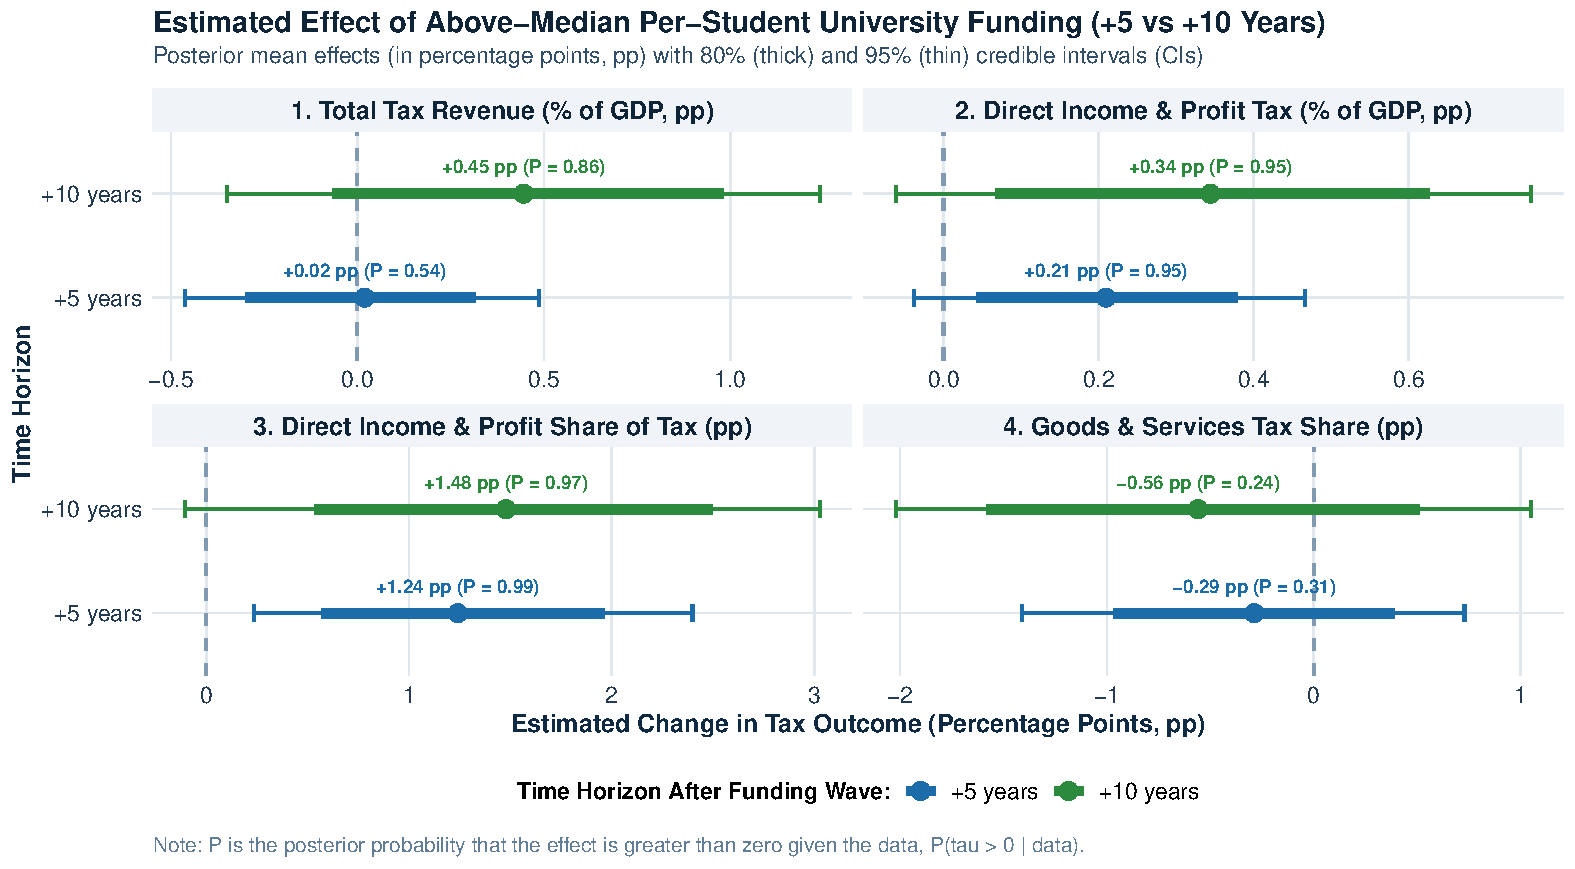
\includegraphics[width=\textwidth]{../outputs/figures/fig2_total_vs_direct_tax_posteriors.pdf}
  \caption{Posterior mean treatment effects (with thick 80\% and thin 95\% credible intervals, CIs) comparing the Total Fiscal Effect (\texttt{M1}, blue) and the Mediator-Removed Direct Fiscal Effect (\texttt{M2}, green) across the four tax outcomes at $+5$ and $+10$ years.}
  \label{fig:posteriors}
\end{figure}

My research suggests three main findings from Table~\ref{tab:main_ate} and Figure~\ref{fig:posteriors}, structured around the two independent dimensions of revenue composition and aggregate tax level:
\begin{enumerate}
  \item \textbf{An Immediate and Lasting Shift Toward Direct Income and Profit Taxation:} Even after separating out forward GDP growth, tertiary enrolment expansion, inequality changes, and life expectancy changes (\texttt{M2}), spending above the income-group benchmark per university student increases the \textbf{Direct Income and Profit Share of Revenue} (Outcome 3) by \textbf{$+1.24$ pp} (95\% CI $[+0.24, +2.40]$, $P = 0.99$, country-clustered $P = 0.99$) at $+5$ years and \textbf{$+1.48$ pp} (95\% CI $[-0.11, +3.03]$, $P = 0.97$, country-clustered $P = 0.96$) at $+10$ years. As explained in Section~\ref{sec:methods}, the mediator-removed direct effect (\texttt{M2}) is slightly larger than the total effect (\texttt{M1}: $+1.02$ pp at $+5\text{y}$ and $+1.36$ pp at $+10\text{y}$), though the paired difference is within one posterior standard deviation, consistent with removing the modest negative suppressor path of short-run student enrolment expansion \citep{kleven2016why, jensen2022employment}.
  \item \textbf{A Decade-Long Maturation Lag for Aggregate Tax-to-GDP and Its Product:} Over the first 5 years, overall \textbf{Non-Resource Tax / GDP} (Outcome 1) barely moves ($+0.02$ pp, 95\% CI $[-0.46, +0.49]$, $P = 0.55$), so the $+5$-year gain of \textbf{$+0.21$ pp of GDP} in \textbf{Direct Income and Profit Tax / GDP} (Outcome 2; 95\% CI $[-0.04, +0.47]$, $P = 0.95$) comes almost entirely from the compositional shift in Outcome 3. By $+10$ years, as university cohorts complete degrees and move into higher-salaried formal careers, overall \textbf{Non-Resource Tax / GDP} rises by $+0.45$ pp of GDP (95\% CI $[-0.35, +1.24]$, $P = 0.86$) and the product channel, \textbf{Direct Income and Profit Tax / GDP}, reaches \textbf{$+0.34$ pp of GDP} (95\% CI $[-0.06, +0.76]$, $P = 0.95$, country-clustered $P = 0.95$; per Equation~\eqref{eq:decomp}, $71\%$ of this $+0.34$ pp gain reflects the compositional shift and $29\%$ reflects aggregate tax-level expansion). Because the 95\% CI for overall Non-Resource Tax / GDP under the binary ratio regime still crosses zero ($[-0.35, +1.24]$), I unbundle the UNESCO denominator in Section~\ref{sec:unbundling}.
  \item \textbf{Weak Evidence of Specificity on Indirect Consumption Taxes:} On the fourth outcome, \textbf{Goods and Services Tax Share}, the estimated direct effect is negative in revenue-share terms at both $+5$ years ($-0.29$ pp, 95\% CI $[-1.41, +0.73]$, $P = 0.31$) and $+10$ years ($-0.56$ pp, 95\% CI $[-2.02, +1.05]$, $P = 0.24$). However, both 95\% CIs are wide and span zero, and as I show in Section~\ref{sec:benchmarks} and Section~\ref{sec:robust}, non-compositional Goods and Services Tax / GDP (\texttt{R11}, $+0.25$ pp, $P = 0.80$) and frequentist benchmarks \texttt{B4} ($+0.72$ pp) and \texttt{B6} ($+0.50$ pp) yield positive point estimates. Thus, the data are largely uninformative on indirect consumption taxes in levels, and the specificity of tertiary education spending shows up in the relative shift of the revenue mix toward direct income and profit taxation rather than an absolute drop in consumption tax receipts.
\end{enumerate}

\subsection{Unbundling the Tertiary Denominator Trap}
\label{sec:unbundling}

Does the fiscal dividend come from spending more \emph{per university student}, or simply from expanding the total university budget as a share of GDP regardless of student numbers? Table~\ref{tab:horserace} and Figure~\ref{fig:horserace} compare my four unbundled tertiary spending definitions side by side at the $+10$-year horizon under the Mediator-Removed Direct Effect specification (\texttt{M2}).

\begin{table}[t!]
  \centering
  \caption{Comparison of $+10$-year Mediator-Removed Direct Fiscal Effects across the four tertiary education spending definitions (with 95\% CIs and posterior probabilities $P = P(\tau > 0 \mid \text{data})$).}
  \label{tab:horserace}
  \small
  \setlength{\tabcolsep}{3.5pt}
  \begin{tabular}{l|c|c|c|c}
    \toprule
    \rowcolor{tabhead}
    \textbf{Tertiary Spending Exposure} & \textbf{$N$ ($C$)} & \textbf{Non-Resource} & \textbf{Direct Income} & \textbf{Direct Income} \\
    \rowcolor{tabhead}
    \textbf{($+10\text{y}$ Direct)} & & \textbf{Tax / GDP (pp)} & \textbf{Tax / GDP (pp)} & \textbf{Tax Share (pp)} \\
    \midrule
    \rowcolor{rowodd}
    \textbf{1. Per-Student Ratio (\texttt{M2b})} & \co 283 (112) & $+0.45$ ($P=0.86$) & \co \textbf{$+0.34$ ($P=0.95$)} & \textbf{$+1.48$ ($P=0.97$)} \\
    \rowcolor{rowodd}
                                                     & \co & {\footnotesize $[-0.35, +1.24]$} & \co {\footnotesize $[-0.06, +0.76]$} & {\footnotesize $[-0.11, +3.03]$} \\
    \hline
    \rowcolor{roweven}
    \textbf{2. Observed Expansion (\texttt{M3b})} & \ce 176 (86) & $+0.53$ ($P=0.82$) & \ce \textbf{$+0.81$ ($P=1.00$)} & \textbf{$+2.33$ ($P=0.99$)} \\
    \rowcolor{roweven}
                                                     & \ce & {\footnotesize $[-0.53, +1.67]$} & \ce {\footnotesize $[+0.29, +1.33]$} & {\footnotesize $[+0.29, +4.36]$} \\
    \hline
    \rowcolor{rowodd}
    \textbf{3. Real PPP \$ / Student (\texttt{M3d})} & \co 283 (112) & \textbf{$+0.94$ ($P=0.99$)} & \co \textbf{$+0.39$ ($P=0.97$)} & $+0.80$ ($P=0.81$) \\
    \rowcolor{rowodd}
                                                     & \co & {\footnotesize $[+0.09, +1.88]$} & \co {\footnotesize $[-0.01, +0.78]$} & {\footnotesize $[-0.91, +2.47]$} \\
    \hline
    \rowcolor{roweven}
    \textbf{4. Tertiary Budget \% GDP (\texttt{M3f})}& \ce 403 (123) & $+0.17$ ($P=0.70$) & \ce $+0.11$ ($P=0.73$) & \textbf{$+0.94$ ($P=0.91$)} \\
    \rowcolor{roweven}
                                                     & \ce & {\footnotesize $[-0.59, +0.83]$} & \ce {\footnotesize $[-0.27, +0.47]$} & {\footnotesize $[-0.37, +2.45]$} \\
    \bottomrule
  \end{tabular}
\end{table}

\begin{figure}[t!]
  \centering
  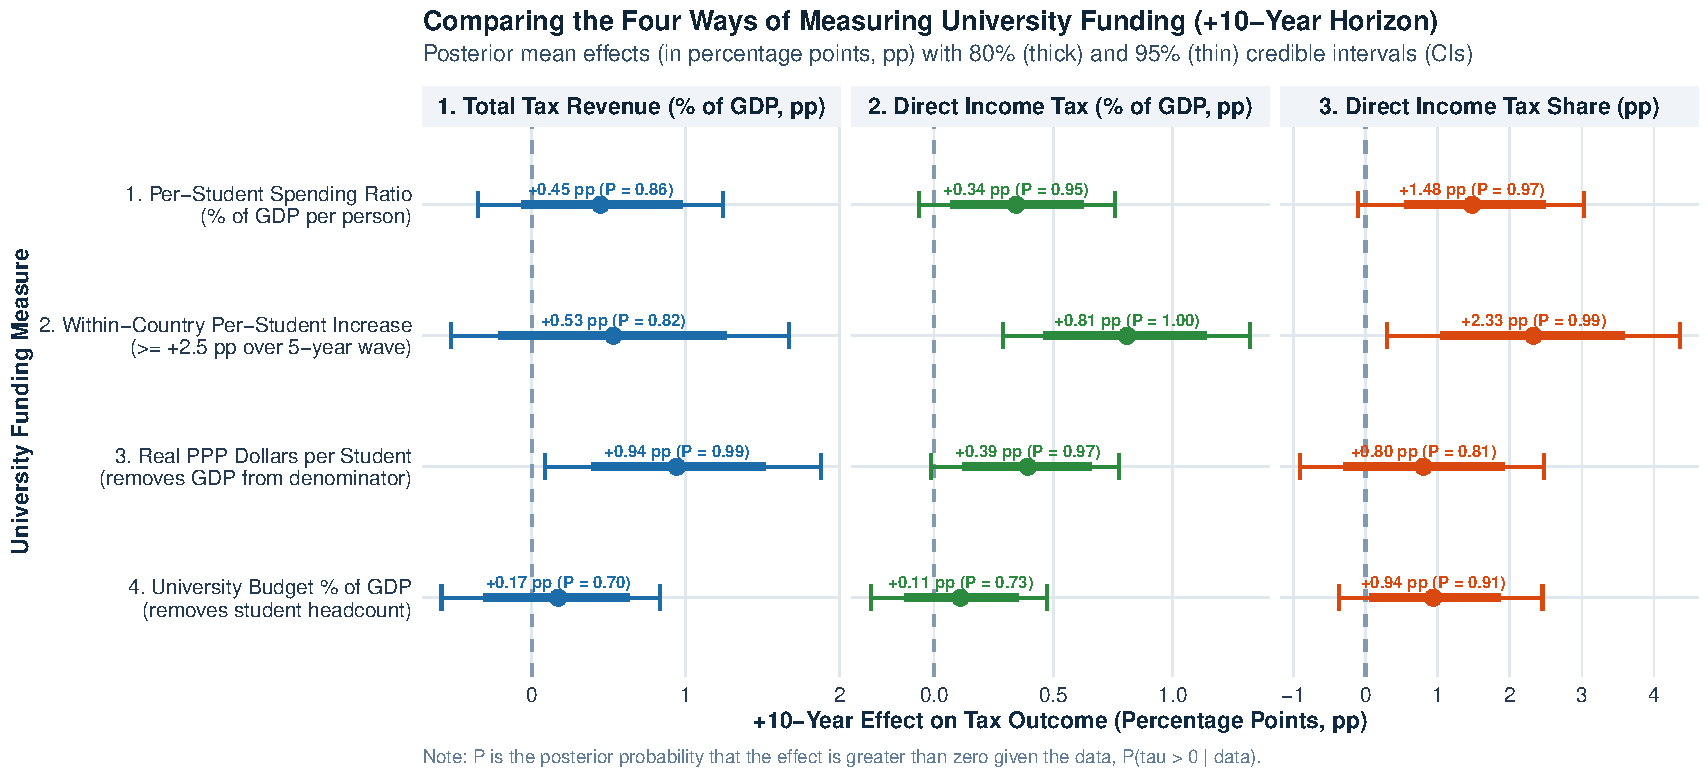
\includegraphics[width=\textwidth]{../outputs/figures/fig3_denominator_unbundling_horserace.pdf}
  \caption{Comparison of $+10$-year Mediator-Removed Direct Fiscal Effects across the four tertiary spending definitions (with country-clustered 95\% and 80\% credible intervals, CIs).}
  \label{fig:horserace}
\end{figure}

Table~\ref{tab:horserace} and Figure~\ref{fig:horserace} show why unbundling the denominator matters so much:
\begin{itemize}
  \item \textbf{Removing GDP from the Denominator Doubles the Total Tax-to-GDP Return:} When I define treatment using \textbf{Real 2021 PPP Dollars per Tertiary Student} (\texttt{M3d}, Row 3), the $+10$-year direct effect on \textbf{Non-Resource Tax / GDP} more than doubles to \textbf{$+0.94$ pp of GDP} (95\% CI $[+0.09, +1.88]$, $P = 0.99$, country-clustered $P = 0.98$), alongside a \textbf{$+0.39$ pp} increase in \textbf{Direct Income Tax / GDP} (95\% CI $[-0.01, +0.78]$, $P = 0.97$).
  \item \textbf{Observed Within-Country Per-Student Expansions Yield the Largest Direct Income Tax Gain:} Comparing country-waves that actually experienced a within-country jump in per-student funding ($\ge +2.5$ pp and $\ge +2.5\%$ over a five-year wave, \texttt{M3b}, Row 2, $N = 176$ across 86 countries) gives a \textbf{$+0.81$ pp of GDP} increase in \textbf{Direct Income and Profit Tax / GDP} (95\% CI $[+0.29, +1.33]$, $P = 1.00$) and a \textbf{$+2.33$ pp} increase in \textbf{Direct Income Tax Share} (95\% CI $[+0.29, +4.36]$, $P = 0.99$), with $+0.53$ pp on overall \textbf{Non-Resource Tax / GDP} (95\% CI $[-0.53, +1.67]$, $P = 0.82$). Even at the $+5$-year horizon (\texttt{M3a}, $N = 253$ across 100 countries), observed per-student expansions raise \textbf{Direct Income Tax / GDP} by \textbf{$+0.28$ pp} (95\% CI $[-0.01, +0.58]$, $P = 0.97$).
  \item \textbf{Per-Student Intensity Matters More Than Unscaled Budget Shares (Including on the Common Sample):} When I remove student headcount from the denominator and look only at the aggregate \textbf{Public Tertiary Budget \% of GDP} (\texttt{M3f}, Row 4, $N = 403$), the $+10$-year effects on Non-Resource Tax / GDP ($+0.17$ pp, 95\% CI $[-0.59, +0.83]$, $P = 0.70$) and Direct Income Tax / GDP ($+0.11$ pp, 95\% CI $[-0.27, +0.47]$, $P = 0.73$) are much weaker. Because Row 4 includes 120 additional country-waves that lack per-student headcount breakdowns, I also verified that restricting \texttt{M2b}, \texttt{M3d}, and \texttt{M3f} to their exact common intersection ($N = 272$ across 108 countries) preserves this ordering: per-student intensity (\texttt{M2b} and \texttt{M3d}) continues to outperform unscaled budget share (\texttt{M3f}), consistent with institutional crowding when student numbers grow faster than funding \citep{bound2010have, deming2017impact, chakrabarti2020state}.
\end{itemize}

\subsection{Heterogeneity by Enrolment Access and Ten-Year Longitudinal Trajectories}

Figure~\ref{fig:moderation} and Table~\ref{tab:subgroups} examine how $+10$-year direct fiscal returns vary across baseline gross tertiary enrolment regimes, all four World Bank income groups, and all five OECD public-versus-private financing regimes.

\begin{figure}[t!]
  \centering
  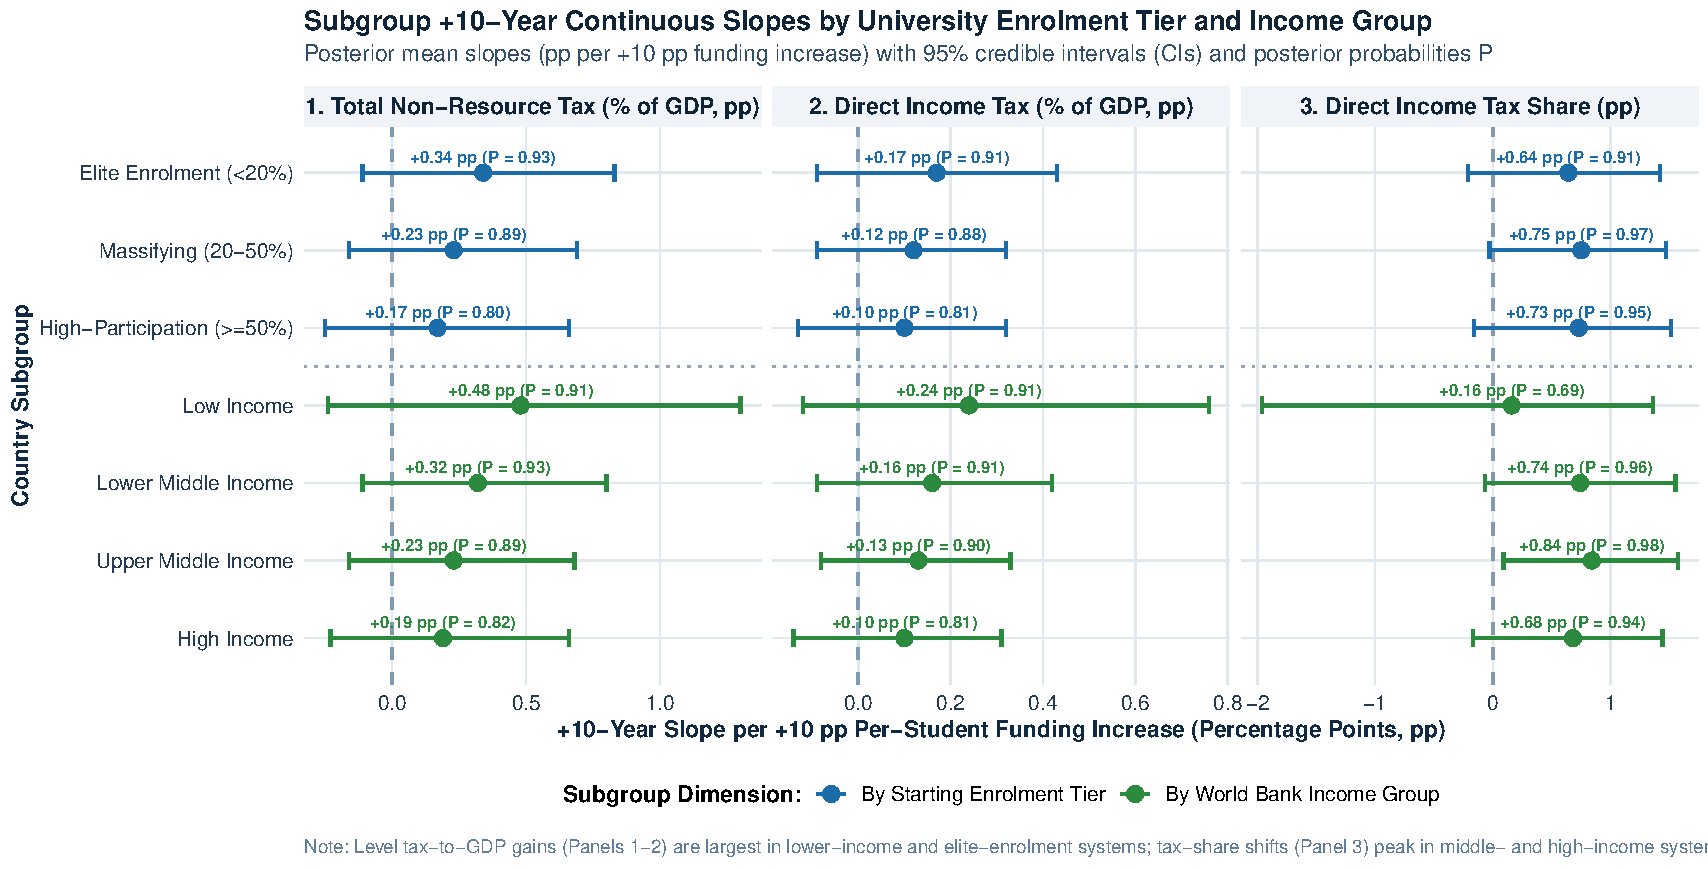
\includegraphics[width=\textwidth]{../outputs/figures/fig4_enrolment_and_oecd_moderation.pdf}
  \caption{Unit-level $+10$-year Mediator-Removed Direct Effect on Direct Income and Profit Tax Share (pp, with vertical 80\% posterior CI bars) across baseline gross tertiary enrolment ratios and World Bank income groups.}
  \label{fig:moderation}
\end{figure}

\begin{table}[t!]
  \centering
  \caption{Subgroup conditional average treatment effects (CATEs, with 95\% CIs on the second line of each cell and posterior probabilities $P = P(\tau > 0 \mid \text{data})$) at the $+10$-year horizon across tertiary enrolment regimes ($N = 244$ observed out of $283$; $39$ waves lack baseline gross enrolment), all four World Bank income groups ($N = 283$), and all five OECD financing tiers ($N = 119$ OECD waves). Subgroups with $N \le 20$ (Row 4 Low Income and Rows 8, 11, 12) are small-sample exploratory strata.}
  \label{tab:subgroups}
  \footnotesize
  \setlength{\tabcolsep}{4.2pt}
  \renewcommand{\arraystretch}{1.12}
  \begin{tabular}{l|c|c|c|c}
    \toprule
    \rowcolor{tabhead}
    \textbf{Subgroup ($+10\text{y}$ Direct)} & \textbf{$N$ ($C$)} & \textbf{Non-Resource} & \textbf{Direct Income} & \textbf{Direct Income} \\
    \rowcolor{tabhead}
    & & \textbf{Tax / GDP (pp)} & \textbf{Tax / GDP (pp)} & \textbf{Tax Share (pp)} \\
    \midrule
    \rowcolor{rowodd}
    \textbf{1. Elite Enrolment ($<20\%$)} & \co 74 (43) & \textbf{$+0.77$ ($P=0.93$)} & \co \textbf{$+0.47$ ($P=0.97$)} & $+0.90$ ($P=0.83$) \\
    \rowcolor{rowodd}
                                               & \co & {\scriptsize $[-0.22, +1.79]$} & \co {\scriptsize $[+0.003, +0.96]$} & {\scriptsize $[-1.07, +2.76]$} \\
    \hline
    \rowcolor{roweven}
    \textbf{2. Massifying ($20\text{--}50\%$)} & \ce 73 (42) & \textbf{$+0.52$ ($P=0.90$)} & \ce \textbf{$+0.35$ ($P=0.94$)} & \textbf{$+1.53$ ($P=0.96$)} \\
    \rowcolor{roweven}
                                               & \ce & {\scriptsize $[-0.32, +1.33]$} & \ce {\scriptsize $[-0.07, +0.76]$} & {\scriptsize $[-0.16, +3.18]$} \\
    \hline
    \rowcolor{rowodd}
    \textbf{3. High-Participation ($\ge 50\%$)}& \co 97 (44) & $+0.22$ ($P=0.68$) & \co $+0.25$ ($P=0.85$) & \textbf{$+1.87$ ($P=0.99$)} \\
    \rowcolor{rowodd}
                                               & \co & {\scriptsize $[-0.77, +1.19]$} & \co {\scriptsize $[-0.23, +0.71]$} & {\scriptsize $[+0.16, +3.63]$} \\
    \hline
    \rowcolor{roweven}
    \textbf{4. Low Income (exploratory)} & \ce 15 (9) & $+0.86$ ($P=0.88$) & \ce \textbf{$+0.56$ ($P=0.97$)} & $-0.03$ ($P=0.54$) \\
    \rowcolor{roweven}
                                               & \ce & {\scriptsize $[-0.54, +2.18]$} & \ce {\scriptsize $[-0.01, +1.23]$} & {\scriptsize $[-3.31, +2.67]$} \\
    \hline
    \rowcolor{rowodd}
    \textbf{5. Lower Middle Income} & \co 47 (21) & \textbf{$+0.79$ ($P=0.94$)} & \co \textbf{$+0.46$ ($P=0.97$)} & $+1.06$ ($P=0.86$) \\
    \rowcolor{rowodd}
                                               & \co & {\scriptsize $[-0.23, +1.86]$} & \co {\scriptsize $[-0.02, +0.96]$} & {\scriptsize $[-0.88, +3.04]$} \\
    \hline
    \rowcolor{roweven}
    \textbf{6. Upper Middle Income} & \ce 76 (35) & \textbf{$+0.61$ ($P=0.93$)} & \ce \textbf{$+0.35$ ($P=0.94$)} & \textbf{$+1.50$ ($P=0.95$)} \\
    \rowcolor{roweven}
                                               & \ce & {\scriptsize $[-0.22, +1.46]$} & \ce {\scriptsize $[-0.09, +0.78]$} & {\scriptsize $[-0.26, +3.23]$} \\
    \hline
    \rowcolor{rowodd}
    \textbf{7. High Income} & \co 145 (47) & $+0.21$ ($P=0.68$) & \co $+0.28$ ($P=0.88$) & \textbf{$+1.76$ ($P=0.99$)} \\
    \rowcolor{rowodd}
                                               & \co & {\scriptsize $[-0.75, +1.09]$} & \co {\scriptsize $[-0.18, +0.74]$} & {\scriptsize $[+0.12, +3.55]$} \\
    \hline
    \rowcolor{roweven}
    \textbf{8. OECD Nordic High-Public} & \ce 20 (5) & $-0.72$ ($P=0.03$) & \ce $-0.01$ ($P=0.50$) & \textbf{$+1.72$ ($P=0.92$)} \\
    \rowcolor{roweven}
                                               & \ce & {\scriptsize $[-1.46, +0.04]$} & \ce {\scriptsize $[-0.68, +0.63]$} & {\scriptsize $[-0.69, +4.11]$} \\
    \hline
    \rowcolor{rowodd}
    \textbf{9. OECD Low-Tuition Public} & \co 46 (15) & $-0.70$ ($P=0.03$) & \co $-0.01$ ($P=0.51$) & \textbf{$+1.69$ ($P=0.92$)} \\
    \rowcolor{rowodd}
                                               & \co & {\scriptsize $[-1.41, +0.03]$} & \co {\scriptsize $[-0.69, +0.62]$} & {\scriptsize $[-0.49, +4.06]$} \\
    \hline
    \rowcolor{roweven}
    \textbf{10. OECD Hybrid Public-Fee} & \ce 29 (8) & $-0.69$ ($P=0.03$) & \ce $-0.03$ ($P=0.48$) & \textbf{$+1.67$ ($P=0.92$)} \\
    \rowcolor{roweven}
                                               & \ce & {\scriptsize $[-1.38, +0.05]$} & \ce {\scriptsize $[-0.71, +0.60]$} & {\scriptsize $[-0.58, +3.99]$} \\
    \hline
    \rowcolor{rowodd}
    \textbf{11. OECD High-Tuition High-Sub.} & \co 11 (5) & $-0.69$ ($P=0.04$) & \co $-0.03$ ($P=0.48$) & \textbf{$+1.67$ ($P=0.92$)} \\
    \rowcolor{rowodd}
                                               & \co & {\scriptsize $[-1.45, +0.08]$} & \co {\scriptsize $[-0.70, +0.62]$} & {\scriptsize $[-0.71, +4.06]$} \\
    \hline
    \rowcolor{roweven}
    \textbf{12. OECD High-Tuition Low-Sub.} & \ce 13 (4) & $-0.63$ ($P=0.04$) & \ce $+0.01$ ($P=0.53$) & \textbf{$+1.65$ ($P=0.91$)} \\
    \rowcolor{roweven}
                                               & \ce & {\scriptsize $[-1.45, +0.10]$} & \ce {\scriptsize $[-0.65, +0.66]$} & {\scriptsize $[-0.76, +4.05]$} \\
    \bottomrule
  \end{tabular}
\end{table}

Figure~\ref{fig:moderation} and Table~\ref{tab:subgroups} reveal an interesting contrast between compositional tax shifts and aggregate tax-to-GDP gains. The shift in revenue composition toward direct income and profit taxation grows steadily with tertiary enrolment access and administrative capacity: $+0.90$ pp in elite systems ($<20\%$ enrolment, $P = 0.83$), \textbf{$+1.53$ pp} in massifying systems ($20\text{--}50\%$ enrolment, $P = 0.96$), and \textbf{$+1.87$ pp} in high-participation systems ($\ge 50\%$ enrolment, 95\% CI $[+0.16, +3.63]$, $P = 0.99$; note that $74 + 73 + 97 = 244$ because $39$ of the $283$ country-waves lack observed baseline gross tertiary enrolment). By contrast, the boost to overall \textbf{Non-Resource Tax / GDP} and \textbf{Direct Income Tax / GDP} is largest in developing and massifying economies where formal tax bases are expanding from a lower starting point: \textbf{Low Income} ($+0.86$ pp on Tax / GDP, $+0.56$ pp on Direct Income Tax / GDP with $P = 0.97$, though with only $N = 15$ across 9 countries its compositional estimate of $-0.03$ pp has a wide CI of $[-3.31, +2.67]$), \textbf{Lower Middle Income} ($+0.79$ pp on Tax / GDP with $P = 0.94$, $+0.46$ pp on Direct Income Tax / GDP with $P = 0.97$), and \textbf{Upper Middle Income} ($+0.61$ pp on Tax / GDP with $P = 0.93$, $+0.35$ pp on Direct Income Tax / GDP with $P = 0.94$), tapering to $+0.21$ pp of GDP in mature \textbf{High Income} economies. In the separate OECD-only sub-model (Rows 8--12, $N = 119$ across 37 countries), all five financing tiers show a positive $+10$-year Direct Income Tax Share CATE ($+1.65$ to $+1.72$ pp, $P \in [0.91, 0.92]$) and near-zero Direct Income Tax / GDP CATE ($-0.03$ to $+0.01$ pp), but negative point estimates on overall Non-Resource Tax / GDP ($-0.63$ to $-0.72$ pp, $P \in [0.03, 0.04]$, 95\% CIs crossing zero at $+0.03$ to $+0.10$ pp). Because these OECD tiers contain only 11 to 46 observations across 4 to 15 countries where per-student public funding is already high across the board (and overall tax-to-GDP already exceeds 35\% of GDP), they cannot support standalone subgroup inference on aggregate tax-to-GDP levels and reflect ceiling effects in mature welfare states.

To see how the fiscal return unfolds step by step within the same country, Table~\ref{tab:lbcf} and Figure~\ref{fig:trajectories} report results from my \textbf{Longitudinal Bayesian Causal Forest (\texttt{lbcf})} fitted on the two stochastic post-baseline transition waves ($+5\text{y}$ and $+10\text{y}$, $2N = 564$ rows) across $N = 282$ complete trajectories (112 countries).

\begin{table}[t!]
  \centering
  \caption{Longitudinal Bayesian Causal Forest decomposition of the initial $+5$-year effect ($\tau_1$), the incremental $+5\text{ to }+10$-year maturation effect ($\tau_2$), the cumulative $+10$-year effect ($\tau_{\text{cum}} = \tau_1 + \tau_2$), and the joint compounding probability $P(\tau_1 > 0 \cap \tau_2 > 0)$, with 95\% CIs on the second line of each cell.}
  \label{tab:lbcf}
  \small
  \setlength{\tabcolsep}{3.6pt}
  \begin{tabular}{l|c|c|c|c}
    \toprule
    \rowcolor{tabhead}
    \textbf{Outcome ($N = 282$)} & \textbf{$+5\text{y}$ Step} & \textbf{$+5\text{--}10\text{y}$ Step} & \textbf{Cumul. $+10\text{y}$} & \textbf{Joint Prob.} \\
    \rowcolor{tabhead}
    & \textbf{($\tau_1$)} & \textbf{($\tau_2$)} & \textbf{($\tau_{\text{cum}}$)} & \textbf{$P(\tau_1>0, \tau_2>0)$} \\
    \midrule
    \rowcolor{rowodd}
    \textbf{1. Non-Resource Tax / GDP} & \co $+0.11$ ($P=0.65$) & $+0.35$ ($P=0.86$) & \co \textbf{$+0.46$ ($P=0.92$)} & 52.7\% \\
    \rowcolor{rowodd}
                                        & \co {\footnotesize $[-0.47, +0.66]$} & {\footnotesize $[-0.29, +1.02]$} & \co {\footnotesize $[-0.14, +1.09]$} & \\
    \hline
    \rowcolor{roweven}
    \textbf{2. Direct Income Tax / GDP} & \ce \textbf{$+0.25$ ($P=0.96$)} & $+0.16$ ($P=0.83$) & \ce \textbf{$+0.41$ ($P=1.00$)} & \textbf{78.8\%} \\
    \rowcolor{roweven}
                                        & \ce {\footnotesize $[-0.04, +0.53]$} & {\footnotesize $[-0.15, +0.50]$} & \ce {\footnotesize $[+0.09, +0.71]$} & \\
    \hline
    \rowcolor{rowodd}
    \textbf{3. Direct Income Tax Share} & \co \textbf{$+1.26$ ($P=0.98$)} & $+0.68$ ($P=0.85$) & \co \textbf{$+1.94$ ($P=1.00$)} & \textbf{83.5\%} \\
    \rowcolor{rowodd}
                                        & \co {\footnotesize $[+0.12, +2.51]$} & {\footnotesize $[-0.61, +2.05]$} & \co {\footnotesize $[+0.76, +3.22]$} & \\
    \hline
    \rowcolor{roweven}
    \textbf{4. Goods \& Services Share} & \ce $-0.59$ ($P=0.18$) & $-0.28$ ($P=0.34$) & \ce $-0.87$ ($P=0.10$) & 2.0\% \\
    \rowcolor{roweven}
                                        & \ce {\footnotesize $[-1.81, +0.79]$} & {\footnotesize $[-1.62, +1.20]$} & \ce {\footnotesize $[-2.22, +0.53]$} & \\
    \bottomrule
  \end{tabular}
\end{table}

\begin{figure}[t!]
  \centering
  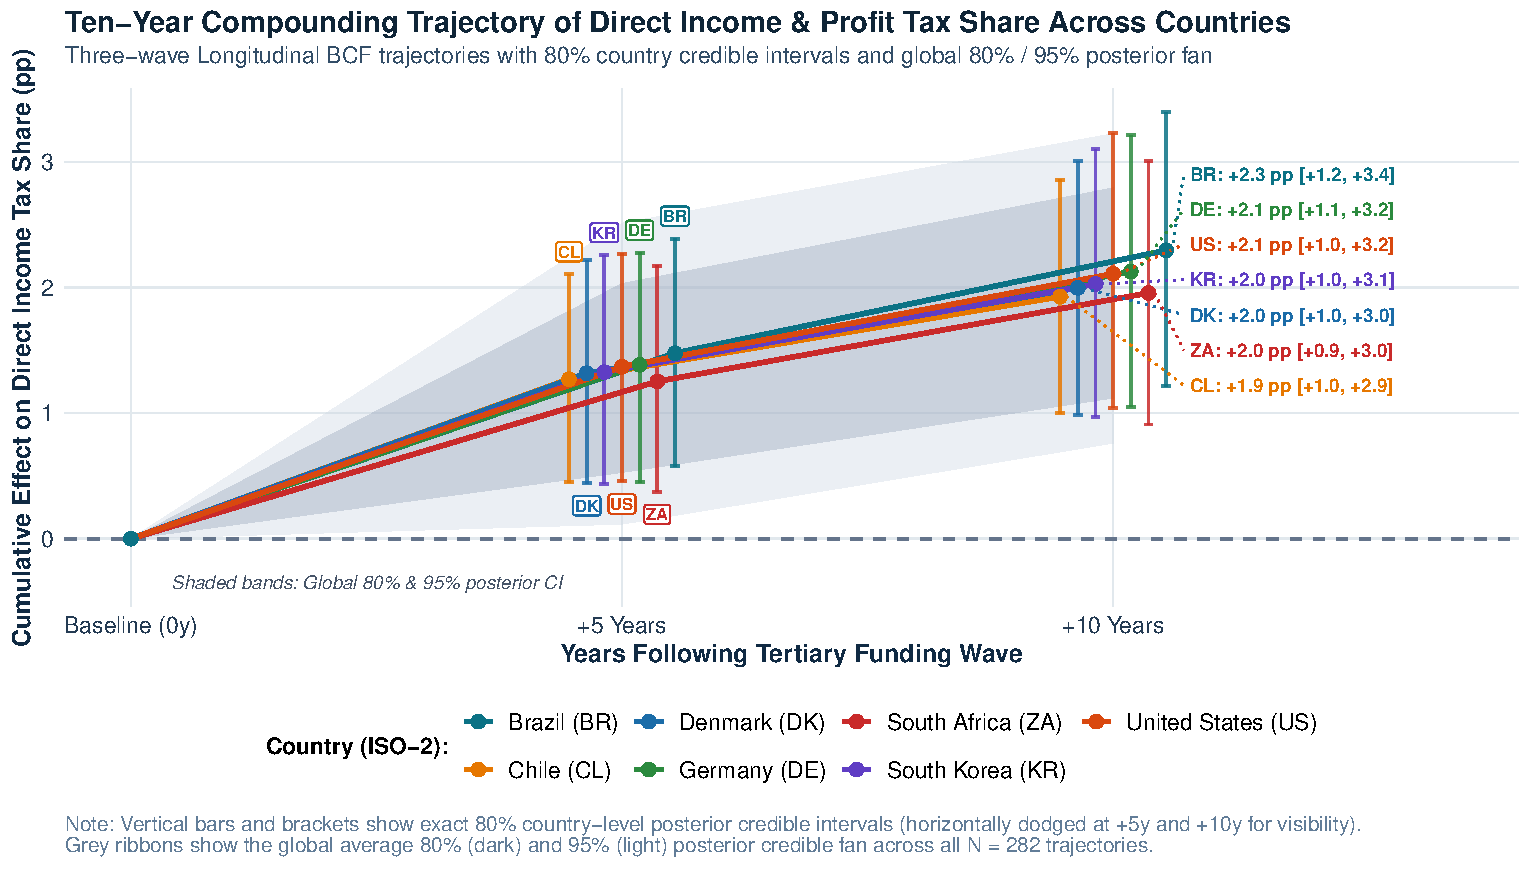
\includegraphics[width=\textwidth]{../outputs/figures/fig5_longitudinal_country_trajectories.pdf}
  \caption{Cumulative 10-year trajectories of the Direct Income and Profit Tax Share effect across seven illustrative countries from the Longitudinal Bayesian Causal Forest, showing country-specific 80\% posterior CIs (vertical bars and brackets, horizontally dodged at $+5$ and $+10$ years for visibility) and the global average 80\% (dark grey) and 95\% (light grey) posterior CI fan.}
  \label{fig:trajectories}
\end{figure}

Table~\ref{tab:lbcf} and Figure~\ref{fig:trajectories} show clear \textbf{ten-year compounding} across the direct fiscal channels once baseline tax levels are differenced out and only the two stochastic post-baseline transition waves are modelled:
\begin{itemize}
  \item On \textbf{Non-Resource Tax / GDP}, an initial $+5$-year gain of $+0.11$ pp (95\% CI $[-0.47, +0.66]$, $P = 0.65$) is followed by a $+0.35$ pp incremental gain between years 5 and 10 (95\% CI $[-0.29, +1.02]$, $P = 0.86$), giving a cumulative 10-year gain of \textbf{$+0.46$ pp of GDP} (95\% CI $[-0.14, +1.09]$, $P = 0.92$, country-clustered $P = 0.92$, with a $52.7\%$ joint posterior probability that both 5-year steps are simultaneously positive).
  \item On \textbf{Direct Income and Profit Tax / GDP}, an initial $+5$-year gain of \textbf{$+0.25$ pp} (95\% CI $[-0.04, +0.53]$, $P = 0.96$) compounds with a $+0.16$ pp gain over years 5 to 10 ($P = 0.83$) to reach \textbf{$+0.41$ pp of GDP} (95\% CI $[+0.09, +0.71]$, $P = 1.00$, joint both-steps-positive probability $78.8\%$).
  \item On \textbf{Direct Income Tax Share}, a \textbf{$+1.26$ pp} gain over years 0 to 5 (95\% CI $[+0.12, +2.51]$, $P = 0.98$) compounds with an additional $+0.68$ pp gain over years 5 to 10 ($P = 0.85$) to reach \textbf{$+1.94$ pp} (95\% CI $[+0.76, +3.22]$, $P = 1.00$, joint both-steps-positive probability $83.5\%$). Pooling both observed post-baseline waves per trajectory ($2N = 564$ transition rows) reduces the posterior SD on cumulative 10-year Direct Income Tax Share from $0.79$ pp in single-horizon \texttt{mvbcf} to $0.64$ pp in \texttt{lbcf} (and from $0.22$ pp to $0.16$ pp on Direct Income Tax / GDP). Figure~\ref{fig:trajectories} plots the global trajectory alongside seven illustrative countries selected to span my running examples (Denmark \texttt{DK}, South Korea \texttt{KR}, and Brazil \texttt{BR}) and four major regional economies from the OECD, Latin America, and Africa (Germany \texttt{DE}, the United States \texttt{US}, Chile \texttt{CL}, and South Africa \texttt{ZA}). Because the conservative $\tau_1$ and $\tau_2$ priors shrink country-level trajectories strongly toward the global curve, the seven country paths cluster tightly between $+1.9$ and $+2.3$ pp at $+10$ years (against country-level 80\% CIs roughly $2.1$ pp wide, such as $+2.3$ pp $[+1.2, +3.4]$ for Brazil and $+2.0$ pp $[+1.0, +3.0]$ for Denmark) and are statistically indistinguishable from one another.
\end{itemize}

\subsection{Causal Method Benchmarks, Ablations, and Moderator Importance}
\label{sec:benchmarks}

As promised in Section~\ref{sec:lit}, I do not want readers to take the performance of the \texttt{mvbcf} model on trust. Table~\ref{tab:benchmarks} compares my primary joint four-outcome \texttt{mvbcf} specification (\texttt{M2b}) at the $+10$-year horizon against two internal ablations and four competing causal estimators fitted on the exact same common sample ($N = 283$, 112 countries).

\begin{table}[t!]
  \centering
  \caption{Method benchmark and ablation comparison at the $+10$-year horizon on the identical common sample ($N = 283$, 112 countries). Posterior means, 95\% Bayesian CIs, and posterior probabilities $P = P(\tau > 0 \mid \text{data})$ are shown for \texttt{mvbcf} and \texttt{B1}--\texttt{B3}; frequentist point estimates, 95\% country-clustered confidence intervals (CI), and one-sided $p$-value complements $P_{\text{freq}} = 1 - p_{\text{one-sided}}$ are shown for \texttt{B4}--\texttt{B6}.}
  \label{tab:benchmarks}
  \footnotesize
  \setlength{\tabcolsep}{1.6pt}
  \begin{tabular}{l|c|c|c|c}
    \toprule
    \rowcolor{tabhead}
    \textbf{Estimator / Ablation ($+10\text{y}$)} & \textbf{Non-Resource} & \textbf{Direct Income} & \textbf{Direct Income} & \textbf{Goods Tax} \\
    \rowcolor{tabhead}
    & \textbf{Tax / GDP} & \textbf{Tax / GDP} & \textbf{Tax Share} & \textbf{Share (Neg. Ctrl)} \\
    \midrule
    \rowcolor{rowodd}
    \textbf{Primary: Joint \texttt{mvbcf} ($D=4$)} & \co $+0.45$ ($P=0.86$) & \textbf{$+0.34$ ($P=0.95$)} & \co \textbf{$+1.48$ ($P=0.97$)} & $-0.56$ ($P=0.24$) \\
    \rowcolor{rowodd}
                                                                & \co {\scriptsize $[-0.35, +1.24]$} & {\scriptsize $[-0.06, +0.76]$} & \co {\scriptsize $[-0.11, +3.03]$} & {\scriptsize $[-2.02, +1.05]$} \\
    \hline
    \rowcolor{roweven}
    \textbf{\texttt{B1}: Univariate BCFs ($D=1$)} & \ce \textbf{$+0.57$ ($P=0.91$)} & \textbf{$+0.39$ ($P=0.97$)} & \ce \textbf{$+1.60$ ($P=0.97$)} & $-0.32$ ($P=0.37$) \\
    \rowcolor{roweven}
                                                                & \ce {\scriptsize $[-0.31, +1.37]$} & {\scriptsize $[-0.01, +0.78]$} & \ce {\scriptsize $[-0.02, +3.28]$} & {\scriptsize $[-2.14, +1.49]$} \\
    \hline
    \rowcolor{rowodd}
    \textbf{\texttt{B2}: \texttt{mvbcf} without $\hat{\pi}(X)$} & \co $+0.45$ ($P=0.87$) & \textbf{$+0.28$ ($P=0.93$)} & \co \textbf{$+1.54$ ($P=0.98$)} & $-0.54$ ($P=0.25$) \\
    \rowcolor{rowodd}
                                                                & \co {\scriptsize $[-0.31, +1.23]$} & {\scriptsize $[-0.09, +0.64]$} & \co {\scriptsize $[+0.09, +3.04]$} & {\scriptsize $[-1.96, +0.97]$} \\
    \hline
    \rowcolor{roweven}
    \textbf{\texttt{B3}: Single-Forest BART} & \ce $+0.28$ ($P=0.80$) & $+0.17$ ($P=0.81$) & \ce \textbf{$+1.05$ ($P=0.94$)} & $-0.38$ ($P=0.30$) \\
    \rowcolor{roweven}
                                                                & \ce {\scriptsize $[-0.34, +0.91]$} & {\scriptsize $[-0.15, +0.53]$} & \ce {\scriptsize $[-0.14, +2.46]$} & {\scriptsize $[-1.92, +1.02]$} \\
    \hline
    \rowcolor{rowodd}
    \textbf{\texttt{B4}: Linear Local Projections} & \co \textbf{$+0.80$ ($P_{\text{freq}}=0.95$)} & $+0.29$ ($P_{\text{freq}}=0.87$) & \co \textbf{$+1.19$ ($P_{\text{freq}}=0.91$)} & $+0.72$ ($P_{\text{freq}}=0.80$) \\
    \rowcolor{rowodd}
                                                                & \co {\scriptsize $[-0.18, +1.79]$} & {\scriptsize $[-0.21, +0.79]$} & \co {\scriptsize $[-0.56, +2.94]$} & {\scriptsize $[-0.97, +2.41]$} \\
    \hline
    \rowcolor{roweven}
    \textbf{\texttt{B5}: Two-Way Fixed Effects} & \ce $-0.26$ ($P_{\text{freq}}=0.33$) & $+0.34$ ($P_{\text{freq}}=0.84$) & \ce \textbf{$+1.55$ ($P_{\text{freq}}=0.92$)} & $-0.13$ ($P_{\text{freq}}=0.46$) \\
    \rowcolor{roweven}
                                                                & \ce {\scriptsize $[-1.40, +0.88]$} & {\scriptsize $[-0.34, +1.01]$} & \ce {\scriptsize $[-0.60, +3.69]$} & {\scriptsize $[-2.79, +2.54]$} \\
    \hline
    \rowcolor{rowodd}
    \textbf{\texttt{B6}: Cross-Fitted Double ML} & \co \textbf{$+1.13$ ($P_{\text{freq}}=0.99$)} & \textbf{$+0.40$ ($P_{\text{freq}}=0.96$)} & \co \textbf{$+1.34$ ($P_{\text{freq}}=0.95$)} & $+0.50$ ($P_{\text{freq}}=0.70$) \\
    \rowcolor{rowodd}
                                                                & \co {\scriptsize $[+0.21, +2.05]$} & {\scriptsize $[-0.06, +0.85]$} & \co {\scriptsize $[-0.30, +2.98]$} & {\scriptsize $[-1.34, +2.34]$} \\
    \bottomrule
  \end{tabular}
\end{table}

Table~\ref{tab:benchmarks} highlights three honest lessons about estimator choice across the four channels:
\begin{enumerate}
  \item \textbf{Modest Differences Across Tree Ablations (\texttt{B1}--\texttt{B3}):} Residual shocks to Direct Income Tax / GDP and Direct Income Tax Share correlate strongly ($r = +0.75$), whilst Income and Goods Tax Shares correlate negatively ($r = -0.58$; Appendix Table~\ref{tab:corr}). Because Outcome 2 is the rescaled product of Outcomes 1 and 3 and Outcome 4 competes in the same revenue denominator as Outcome 3, part of this residual correlation is algebraic rather than purely macroeconomic; jointly modelling $\Sigma$ yields a modest ($\approx 7\%$) reduction in posterior standard deviation ($0.79$ pp in \texttt{mvbcf} vs $0.85$ pp in univariate \texttt{B1} on Direct Income Tax Share), whilst univariate BCFs (\texttt{B1}) yield slightly larger point estimates ($+0.57$ pp on Tax / GDP and $+1.60$ pp on Direct Income Tax Share). Similarly, dropping $\hat{\pi}(X_{i,t})$ (\texttt{B2}, $+0.28$ pp on Direct Income Tax / GDP) or fitting a single-forest BART without separate $(\mu, \tau)$ shrinkage (\texttt{B3}, $+0.17$ pp on Direct Income Tax / GDP and $+1.05$ pp on Direct Income Tax Share) shifts the point estimates downward in the direction predicted by \citet{hahn2020bayesian}, though these differences remain smaller than one posterior standard deviation ($\approx 0.22$ pp and $0.79$ pp) and are not statistically distinguishable at $N = 283$.
  \item \textbf{Substantial Estimator Disagreement on Aggregate Tax-to-GDP vs Strong Agreement on Composition (\texttt{B4}--\texttt{B6}):} The most striking pattern in Table~\ref{tab:benchmarks} is the contrast between Outcome 1 and Outcomes 2--3 across the frequentist benchmarks. On aggregate \textbf{Non-Resource Tax / GDP} (Outcome 1), the six estimators span a wide range from \textbf{$-0.26$ pp} under country-and-wave Two-Way Fixed Effects (\texttt{B5}, $95\%$ CI $[-1.40, +0.88]$) to \textbf{$+0.80$ pp} under Linear Local Projections (\texttt{B4}; \citealt{jorda2005estimation}) and \textbf{$+1.13$ pp} under 5-fold country-blocked Cross-Fitted Double ML (\texttt{B6}; \citealt{chernozhukov2018double}). By contrast, on \textbf{Direct Income Tax Share} (Outcome 3) and \textbf{Direct Income Tax / GDP} (Outcome 2), every estimator in Table~\ref{tab:benchmarks} agrees on the sign and approximate magnitude: Direct Income Tax Share ranges tightly from $+1.05$ to $+1.60$ pp (with $+1.19$ pp in \texttt{B4}, $+1.55$ pp in \texttt{B5}, and $+1.34$ pp in \texttt{B6}) and Direct Income Tax / GDP ranges from $+0.17$ to $+0.40$ pp ($+0.29$ pp in \texttt{B4}, $+0.34$ pp in \texttt{B5}, and $+0.40$ pp in \texttt{B6}). Meanwhile, Goods Tax Share (Outcome 4) flips sign to $+0.72$ pp in \texttt{B4} and $+0.50$ pp in \texttt{B6}. This comparison shows that while aggregate tax-to-GDP level estimates are sensitive to functional form and fixed-effect specification, the compositional shift toward direct income taxation is stable across all six estimators.
\end{enumerate}

Following \citet{woody2021model}, I also project the unit-level CATE posterior draws onto the 8-variable moderator matrix $W_{i,t}$ to see which country characteristics drive treatment-effect heterogeneity. Together, the linear surrogate projection explains $R^2_{\text{total}} = 58.4\%$ of systematic CATE variation across the four outcomes, of which $33.4\%$ reflects shared collinear variation across correlated development indicators and $25.0\%$ reflects the sum of unique orthogonal partial-$R^2$ contributions from individual moderators: \textbf{baseline log real GDP per person} (unique partial $R^2 = 8.1\%$, correlating at $r = -0.71$ with Non-Resource Tax / GDP CATEs and $r = +0.76$ with Direct Income Tax Share CATEs), \textbf{working-age population share} ($6.1\%$, correlating at $r = +0.75$ with Direct Income Tax Share CATEs), \textbf{baseline gross tertiary enrolment} ($3.7\%$, correlating at $r = -0.59$ with Direct Income Tax / GDP CATEs and $r = +0.67$ with Direct Income Tax Share CATEs), \textbf{OECD membership} ($3.7\%$, correlating at $r = -0.82$ with Goods Tax Share CATEs), and \textbf{baseline direct income tax share} ($3.4\%$).

\subsection{Robustness, Sensitivity, and Falsification Checks (\texttt{R1} to \texttt{R12})}
\label{sec:robust}

Table~\ref{tab:robust} summarises 13 sensitivity, identification, and falsification checks (\texttt{R1} to \texttt{R12}, with \texttt{R3} evaluated at both $+5\text{y}$ and $+10\text{y}$) testing data construction, decadal wave overlap, country fixed effects at both horizons, strictly observed covariates, pre-treatment placebo trends, $\tau$-forest prior specification, SWIID inequality measurement error, country-blocked out-of-fold preprocessing, two-stage sequential g-estimation, pre-treatment fiscal trend controls, non-compositional consumption tax negative controls, and pre-COVID sample restriction.

\begin{table}[t!]
  \centering
  \caption{Robustness, identification, and falsification checks across the primary fiscal outcomes (with 95\% CIs on the second line of each cell and posterior probabilities $P = P(\tau > 0 \mid \text{data})$).}
  \label{tab:robust}
  \footnotesize
  \setlength{\tabcolsep}{3.2pt}
  \renewcommand{\arraystretch}{1.15}
  \begin{tabular}{l|c|c|c|c}
    \toprule
    \rowcolor{tabhead}
    \textbf{Specification} & \textbf{Horizon ($N, C$)} & \textbf{Non-Resource} & \textbf{Direct Income} & \textbf{Direct Income} \\
    \rowcolor{tabhead}
    & & \textbf{Tax / GDP (pp)} & \textbf{Tax / GDP (pp)} & \textbf{Tax Share (pp)} \\
    \midrule
    \rowcolor{rowodd}
    \textbf{\texttt{R1}. Pure WDI Tax / GDP} & \co $+10\text{y}$ (283, 112) & $+0.34$ ($P=0.79$) & \co \textbf{$+0.30$ ($P=0.94$)} & \textbf{$+1.48$ ($P=0.97$)} \\
    \rowcolor{rowodd}
                                                      & \co & {\scriptsize $[-0.42, +1.08]$} & \co {\scriptsize $[-0.10, +0.70]$} & {\scriptsize $[-0.04, +3.01]$} \\
    \hline
    \rowcolor{roweven}
    \textbf{\texttt{R2}. Non-Overlapping 10y Waves} & \ce $+10\text{y}$ (154, 105) & \textbf{$+0.64$ ($P=0.91$)} & \ce \textbf{$+0.36$ ($P=0.93$)} & \textbf{$+1.96$ ($P=0.98$)} \\
    \rowcolor{roweven}
                                                      & \ce & {\scriptsize $[-0.31, +1.56]$} & \ce {\scriptsize $[-0.10, +0.81]$} & {\scriptsize $[+0.09, +3.92]$} \\
    \hline
    \rowcolor{rowodd}
    \textbf{\texttt{R3a}. Country Fixed Effects ($+5\text{y}$)} & \co $+5\text{y}$ (372, 121) & $+0.08$ ($P=0.62$) & \co \textbf{$+0.19$ ($P=0.93$)} & \textbf{$+0.96$ ($P=0.97$)} \\
    \rowcolor{rowodd}
                                                      & \co & {\scriptsize $[-0.43, +0.56]$} & \co {\scriptsize $[-0.06, +0.43]$} & {\scriptsize $[-0.06, +2.00]$} \\
    \hline
    \rowcolor{roweven}
    \textbf{\texttt{R3b}. Country Fixed Effects ($+10\text{y}$)} & \ce $+10\text{y}$ (283, 112) & $+0.32$ ($P=0.82$) & \ce $+0.15$ ($P=0.79$) & $+0.69$ ($P=0.84$) \\
    \rowcolor{roweven}
                                                      & \ce & {\scriptsize $[-0.34, +0.97]$} & \ce {\scriptsize $[-0.20, +0.51]$} & {\scriptsize $[-0.63, +2.06]$} \\
    \hline
    \rowcolor{rowodd}
    \textbf{\texttt{R4}. Strictly Observed Covariates}& \co $+10\text{y}$ (238, 107) & \textbf{$+0.56$ ($P=0.92$)} & \co \textbf{$+0.38$ ($P=0.98$)} & \textbf{$+1.94$ ($P=0.99$)} \\
    \rowcolor{rowodd}
                                                      & \co & {\scriptsize $[-0.22, +1.30]$} & \co {\scriptsize $[+0.01, +0.81]$} & {\scriptsize $[+0.36, +3.60]$} \\
    \hline
    \rowcolor{roweven}
    \textbf{\texttt{R5}. Placebo ($\Delta Y_{t-1\to t}$)}& \ce Pre-$t$ (348, 117) & $+0.24$ ($P=0.79$) & \ce $+0.07$ ($P=0.66$) & $+0.59$ ($P=0.83$) \\
    \rowcolor{roweven}
                                                      & \ce & {\scriptsize $[-0.34, +0.79]$} & \ce {\scriptsize $[-0.21, +0.35]$} & {\scriptsize $[-0.55, +1.68]$} \\
    \hline
    \rowcolor{rowodd}
    \textbf{\texttt{R6}. Diffuse $\tau$ Prior} & \co $+10\text{y}$ (283, 112) & $+0.47$ ($P=0.89$) & \co \textbf{$+0.29$ ($P=0.91$)} & \textbf{$+1.67$ ($P=0.98$)} \\
    \rowcolor{rowodd}
                                                      & \co & {\scriptsize $[-0.27, +1.19]$} & \co {\scriptsize $[-0.13, +0.71]$} & {\scriptsize $[+0.03, +3.16]$} \\
    \hline
    \rowcolor{roweven}
    \textbf{\texttt{R7}. SWIID Error Perturbation} & \ce $+10\text{y}$ (283, 112) & \textbf{$+0.55$ ($P=0.90$)} & \ce \textbf{$+0.26$ ($P=0.90$)} & \textbf{$+1.49$ ($P=0.97$)} \\
    \rowcolor{roweven}
                                                      & \ce & {\scriptsize $[-0.27, +1.38]$} & \ce {\scriptsize $[-0.14, +0.66]$} & {\scriptsize $[-0.01, +2.99]$} \\
    \hline
    \rowcolor{rowodd}
    \textbf{\texttt{R8}. Country-Blocked OOF PS} & \co $+10\text{y}$ (283, 112) & \textbf{$+0.55$ ($P=0.93$)} & \co \textbf{$+0.26$ ($P=0.91$)} & \textbf{$+1.49$ ($P=0.98$)} \\
    \rowcolor{rowodd}
                                                      & \co & {\scriptsize $[-0.15, +1.28]$} & \co {\scriptsize $[-0.14, +0.64]$} & {\scriptsize $[+0.04, +2.94]$} \\
    \hline
    \rowcolor{roweven}
    \textbf{\texttt{R9}. Sequential G-Estimation} & \ce $+10\text{y}$ (283, 112) & \textbf{$+0.70$ ($P=0.97$)} & \ce \textbf{$+0.39$ ($P=0.97$)} & \textbf{$+1.51$ ($P=0.99$)} \\
    \rowcolor{roweven}
                                                      & \ce & {\scriptsize $[-0.02, +1.47]$} & \ce {\scriptsize $[-0.002, +0.78]$} & {\scriptsize $[+0.18, +2.97]$} \\
    \hline
    \rowcolor{rowodd}
    \textbf{\texttt{R10}. Pre-Trend Controls ($\Delta Y_{t-1\to t}$)} & \co $+10\text{y}$ (283, 112) & $+0.44$ ($P=0.85$) & \co \textbf{$+0.32$ ($P=0.93$)} & \textbf{$+1.68$ ($P=0.98$)} \\
    \rowcolor{rowodd}
                                                      & \co & {\scriptsize $[-0.37, +1.21]$} & \co {\scriptsize $[-0.08, +0.72]$} & {\scriptsize $[+0.11, +3.14]$} \\
    \hline
    \rowcolor{roweven}
    \textbf{\texttt{R11}. Goods Tax / GDP Neg. Ctrl} & \ce $+10\text{y}$ (283, 112) & \textbf{$+0.54$ ($P=0.92$)} & \ce \textbf{$+0.30$ ($P=0.94$)} & \textbf{$+1.42$ ($P=0.96$)} \\
    \rowcolor{roweven}
                                                      & \ce & {\scriptsize $[-0.23, +1.33]$} & \ce {\scriptsize $[-0.09, +0.73]$} & {\scriptsize $[-0.21, +3.13]$} \\
    \hline
    \rowcolor{rowodd}
    \textbf{\texttt{R12}. Pre-COVID Sample ($<2020$)} & \co $+10\text{y}$ (187, 90) & \textbf{$+0.71$ ($P=0.92$)} & \co $+0.17$ ($P=0.71$) & $+0.74$ ($P=0.77$) \\
    \rowcolor{rowodd}
                                                      & \co & {\scriptsize $[-0.30, +1.75]$} & \co {\scriptsize $[-0.35, +0.70]$} & {\scriptsize $[-1.30, +2.71]$} \\
    \bottomrule
  \end{tabular}
\end{table}

The checks in Table~\ref{tab:robust} show both where my findings are robust and where care is needed:
\begin{itemize}
  \item \textbf{Pure WDI Tax-to-GDP (\texttt{R1}) and Non-Overlapping Decadal Waves (\texttt{R2}):} Replacing resource-adjusted tax revenue with raw WDI tax-to-GDP (\texttt{R1}) leaves Direct Income Tax / GDP ($+0.30$ pp, $P = 0.94$) and Direct Income Tax Share ($+1.48$ pp, $P = 0.97$) unchanged. Restricting the sample to strictly non-overlapping 10-year decadal waves (\texttt{1990--1994}, \texttt{2000--2004}, \texttt{2010--2014}, \texttt{2020--2024}; \texttt{R2}, $N = 154$) removes moving-average overlap and strengthens the $+10$-year effects to \textbf{$+0.64$ pp} on Non-Resource Tax / GDP ($P = 0.91$), \textbf{$+0.36$ pp} on Direct Income Tax / GDP ($P = 0.93$), and \textbf{$+1.96$ pp} on Direct Income Tax Share (95\% CI $[+0.09, +3.92]$, $P = 0.98$).
  \item \textbf{Within-Country Demeaning (\texttt{R3a}, \texttt{R3b}) and Strictly Observed Covariates (\texttt{R4}):} Demeaning every outcome within each country absorbs time-invariant national institutions, giving \textbf{$+0.19$ pp} ($P = 0.93$) on Direct Income Tax / GDP and \textbf{$+0.96$ pp} ($P = 0.97$) on Direct Income Tax Share at $+5$ years (\texttt{R3a}). I want to be honest about \texttt{R3b}: at $+10$ years, demeaning a persistent binary regime indicator across an average of only $2.5$ waves per country attenuates the estimates ($+0.32$ pp on Non-Resource Tax / GDP, $P = 0.82$; $+0.15$ pp on Direct Income Tax / GDP, $P = 0.79$; $+0.69$ pp on Direct Income Tax Share, $P = 0.84$). That is why pairing the regime contrast with my observed within-country expansion treatment (\texttt{M3b} in Table~\ref{tab:horserace}, which gives $+0.81$ pp on Direct Income Tax / GDP, $P = 1.00$) is so important. Dropping all country-waves with any imputed baseline covariate (\texttt{R4}, $N = 238$) increases $+10$-year Direct Income Tax / GDP to \textbf{$+0.38$ pp} (95\% CI $[+0.01, +0.81]$, $P = 0.98$) and Direct Income Tax Share to \textbf{$+1.94$ pp} (95\% CI $[+0.36, +3.60]$, $P = 0.99$).
  \item \textbf{Placebo Pre-Trend Test (\texttt{R5}) and Explicit Pre-Trend Controls (\texttt{R10}):} Testing whether wave-$t$ tertiary funding predicts \emph{past, pre-treatment} fiscal changes ($\Delta Y_{i, t-1 \to t}$, \texttt{R5}, $N = 348$) yields $+0.07$ pp on Direct Income Tax / GDP (95\% CI $[-0.21, +0.35]$, $P = 0.66$) and $+0.24$ pp on Non-Resource Tax / GDP (95\% CI $[-0.34, +0.79]$, $P = 0.79$), but a non-trivial \textbf{$+0.59$ pp} pre-trend on Direct Income Tax Share (95\% CI $[-0.55, +1.68]$, $P = 0.83$, roughly half the $+5$-year effect). Specification \texttt{R10} directly tests whether this pre-treatment trend drives the post-treatment result: when I explicitly include all four pre-treatment fiscal trends $\Delta Y_{i, t-1 \to t}$ in $X_{i,t}$ (\texttt{R10}), $+10$-year Direct Income Tax / GDP remains \textbf{$+0.32$ pp} ($P = 0.93$) and Direct Income Tax Share increases slightly to \textbf{$+1.68$ pp} (95\% CI $[+0.11, +3.14]$, $P = 0.98$), confirming that the $+10$-year compositional shift is not an artefact of pre-existing fiscal trajectories.
  \item \textbf{Prior Sensitivity (\texttt{R6}), Inequality Measurement Error (\texttt{R7}), Out-of-Fold Preprocessing (\texttt{R8}), Sequential G-Estimation (\texttt{R9}), and Non-Compositional Negative Control (\texttt{R11}):} Relaxing the $\tau$-forest prior to $\alpha_\tau = 0.50, M_\tau = 50$ (\texttt{R6}), propagating country-year-specific SWIID standard errors (\texttt{R7}), and running strictly out-of-fold country-blocked median imputation and propensity estimation (\texttt{R8}) all preserve the $+10$-year Direct Income Tax Share dividend ($+1.67$ pp, $+1.49$ pp, and $+1.49$ pp, all $P \ge 0.97$). Removing mediator effects via two-stage sequential g-estimation \citep{acharya2016explaining} (\texttt{R9}) yields \textbf{$+0.70$ pp} on Non-Resource Tax / GDP ($P = 0.97$), \textbf{$+0.39$ pp} on Direct Income Tax / GDP (95\% CI $[-0.002, +0.78]$, $P = 0.97$), and \textbf{$+1.51$ pp} on Direct Income Tax Share (95\% CI $[+0.18, +2.97]$, $P = 0.99$). When I replace compositional Goods Tax Share with non-compositional \textbf{Goods and Services Tax / GDP} (\texttt{R11}), Goods Tax / GDP also rises slightly by $+0.25$ pp (95\% CI $[-0.32, +0.80]$, $P = 0.80$) alongside $+0.30$ pp ($P = 0.94$) on Direct Income Tax / GDP, indicating that in GDP levels treated countries collect somewhat more across both bases and that specificity operates through the relative revenue mix.
  \item \textbf{Pre-COVID Sample Restriction (\texttt{R12}):} Dropping the \texttt{2020--2024} outcome wave (\texttt{R12}, $N = 187$ across 90 countries) reveals an important difference between the pre-pandemic and full samples. Without \texttt{2020--2024}, the $+10$-year point estimate on aggregate \textbf{Non-Resource Tax / GDP} strengthens from $+0.45$ pp ($P = 0.86$) to \textbf{$+0.71$ pp} (95\% CI $[-0.30, +1.75]$, $P = 0.92$), whereas the compositional \textbf{Direct Income Tax Share} estimate roughly halves from $+1.48$ pp ($P = 0.97$) to \textbf{$+0.74$ pp} (95\% CI $[-1.30, +2.71]$, $P = 0.77$) and \textbf{Direct Income Tax / GDP} halves from $+0.34$ pp ($P = 0.95$) to \textbf{$+0.17$ pp} (95\% CI $[-0.35, +0.70]$, $P = 0.71$). In other words, the pre-2020 sample exhibits a larger aggregate revenue gain but a smaller and less precise compositional shift. I discuss the substantive economic and pandemic-era mechanisms behind this finding in Section~\ref{sec:discussion}.
\end{itemize}

\section{Mechanisms, Limitations, and Future Directions}
\label{sec:discussion}

\subsection{Cohort Maturation Timelines and Practical Policy Lessons}

How does government spending on universities start shifting tax composition within $+5$ years ($+1.24$ pp on Direct Income Tax Share; $+0.21$ pp on Direct Income Tax / GDP) before building over $+10$ years ($+0.34$ to $+0.81$ pp on Direct Income Tax / GDP and $+0.45$ to $+0.94$ pp on Non-Resource Tax / GDP)? Three mechanisms help explain the pattern of results across horizons and samples:
\begin{enumerate}
  \item \textbf{Immediate Institutional Withholding ($+5$ Years), Graduate Career Maturation ($+10$ Years), and Pandemic Resilience (\texttt{R12}):} Because the panel aggregates annual data into five-year waves, a funding increase in wave $t$ (spanning years 0 to 4) is evaluated in wave $t+1$ (years 5 to 9) and wave $t+2$ (years 10 to 14). In the first five-year window, higher per-student university spending immediately expands formal university payrolls (academic staff, researchers, and administrators subject to automatic PAYE income tax withholding) whilst students enrolled in three-year bachelor's and one-to-two-year master's programmes enter their first formal jobs. By the $+10$-year window (years 10 to 14), two university cohorts have graduated and moved into prime-age managerial, professional, and technical roles \citep{kleven2016why, jensen2022employment, moretti2004estimating, valero2019economic}. At the same time, \texttt{R12} shows that roughly half of the $+10$-year compositional shift toward direct income tax share ($+1.48$ pp full sample vs $+0.74$ pp pre-COVID) comes from the \texttt{2020--2024} outcome wave. A plausible explanation is that during the 2020--2021 COVID-19 shock, lockdowns and retail closures sharply depressed indirect consumption (VAT) bases, whereas salaried graduate and professional employment (which is larger in countries that invested heavily in universities a decade earlier) shifted smoothly to remote work and was protected by formal furlough schemes and automatic payroll withholding. Thus, the full-sample compositional effect reflects both gradual graduate formalisation and the greater resilience of direct income tax bases relative to consumption taxes during the pandemic.
  \item \textbf{Protecting Per-Student Resources and Comparing Fiscal Magnitudes:} My denominator unbundling in Section~\ref{sec:unbundling} shows that expanding total university budgets without protecting per-student funding intensity yields weak fiscal returns ($+0.11$ pp on Direct Income Tax / GDP in \texttt{M3f}). Countries that maintain or expand real resources \emph{per student} (\texttt{M2b}, \texttt{M3b}, \texttt{M3d}) avoid institutional crowding \citep{bound2010have, deming2017impact, chakrabarti2020state} and collect more future direct tax. To put these magnitudes in perspective using Table~\ref{tab:eda1}, median public tertiary budgets stand at $0.47\%$ to $0.94\%$ of GDP across income groups, so a $25\%$ to $35\%$ relative expansion in per-student funding corresponds to roughly $0.15$ to $0.30$ pp of GDP in annual public expenditure. Over a 10-year horizon, the estimated direct income tax gains ($+0.34$ pp of GDP under the ratio regime and $+0.81$ pp under observed within-country expansions) and non-resource tax gains ($+0.45$ to $+0.94$ pp of GDP) are of the \textbf{same order of magnitude} as the upfront budgetary flow \citep{hendren2020unified}, though because the primary $+10$-year 95\% CI on aggregate Non-Resource Tax / GDP crosses zero ($[-0.35, +1.24]$) and formal fiscal accounting requires discounting annual cost and revenue flows over cohort careers, these estimates should be interpreted as evidence of substantial partial fiscal recoupment rather than a guaranteed net fiscal surplus.
  \item \textbf{Where the Upside Is Largest:} Returning to my running example, developing and massifying countries (like Brazil, Chile, or South Africa) expanding from elite ($<20\%$) to massifying ($20\text{--}50\%$) university systems see the largest point estimates in direct income tax capacity ($+0.35$ to $+0.56$ pp of GDP) and total non-resource tax capacity ($+0.52$ to $+0.86$ pp of GDP), whereas mature high-income economies (like Denmark) exhibit a compositional shift toward direct income taxation ($+1.76$ pp of revenue) with no detectable change in the aggregate tax-to-GDP level ($+0.21$ pp, 95\% CI $[-0.75, +1.09]$, $P = 0.68$).
\end{enumerate}

\subsection{Limitations and Future Research}

Several caveats apply when interpreting observational cross-country macro panels:
\begin{enumerate}
  \item \textbf{Reverse causality and fiscal-capacity feedback:} A central threat in macro-fiscal panels is that growing tax capacity enables governments to spend more on higher education rather than the other way round \citep{baumol1967macroeconomics, worldbank2024taxing, unesco2024efw}. In particular, \citet{worldbank2024taxing} show that countries crossing the 15\% tax-to-GDP threshold subsequently expand public health and education budgets. Whilst I condition on baseline tax-to-GDP, baseline income and goods tax shares, lagged GDP growth, and explicit pre-treatment fiscal trends $\Delta Y_{i, t-1 \to t}$ (\texttt{R10}), observational conditioning cannot completely rule out multi-decade fiscal-capacity feedback loops.
  \item \textbf{Unobserved concurrent reforms:} My identification of the total effect (\texttt{M1}) relies on conditional ignorability given the 19 baseline covariates and lagged growth, whilst the mediator-removed direct effect (\texttt{M2}) and sequential g-estimator (\texttt{R9}) assume sequential ignorability of the four post-treatment mediators \citep{imai2010general, acharya2016explaining}. If a reformist government simultaneously overhauls its electronic tax administration \citep{pomeranz2019taking, okunogbe2022technology} and increases university funding in the same five-year wave, part of my estimated direct effect could reflect that concurrent tax reform.
  \item \textbf{Skilled emigration (brain drain):} In small low- and lower-middle-income countries, a substantial share of university graduates emigrate to richer economies \citep{beine2008brain}. Because emigrants pay direct income taxes in their destination country whilst sending untaxed remittances home (which are spent on domestic goods subject to VAT), high skilled emigration can dampen domestic direct income tax returns whilst propping up consumption tax shares.
  \item \textbf{Central versus general government tax boundaries and five-year wave coarseness:} WDI fiscal series mainly record central government budgetary revenue, which can understate state or provincial income taxes in federal countries. Similarly, averaging annual series into five-year waves smooths out business-cycle noise and handles patchy UNESCO reporting, but blurs year-by-year timing and restricts the complete four-outcome sample to 121 countries.
\end{enumerate}

These limitations point to several concrete avenues for future work:
\begin{itemize}
  \item Extending longitudinal Bayesian causal forests to 15-to-25-year horizons so that researchers can compare government spending on early childhood, primary, and secondary schooling \citep{hanushek2012better, angrist2021measuring} directly against tertiary education as school-age cohorts reach adulthood.
  \item Incorporating bilateral skilled migration matrices \citep{beine2008brain} as an explicit moderator in $\tau(W_{i,t})$ to measure how brain drain alters the fiscal return to public university subsidies in developing economies.
  \item Linking university funding cohorts directly to administrative employer-employee tax registers within individual countries to track graduate earnings and firm corporate tax payments year by year.
\end{itemize}

\section*{Declarations and Statements}

\paragraph{Author Contributions (CRediT).}
\textbf{Andrew C. Parnell:} Conceptualisation, Data curation, Formal analysis, Methodology, Software, Visualisation, Writing -- original draft, Writing -- review and editing.

\paragraph{Data Availability Statement.}
All raw and processed datasets analysed in this study are derived from publicly available international databases (World Bank WDI, UNESCO UIS, IMF, WGI, SWIID, and OECD) licensed under CC-BY-4.0 and are included in the project repository at \url{https://github.com/andrewcparnell/education-tax-bcf} (with full SHA-256 checksums and provenance documented in \texttt{data/raw/PROVENANCE.md}).

\paragraph{Code Availability Statement.}
All R and C++ (\texttt{RcppArmadillo}) source code, data-cleaning scripts, MCMC samplers, diagnostic scripts, interactive exploration app (\texttt{app/}), automated pipeline tests, and figure generation pipelines are openly available under the MIT License at \url{https://github.com/andrewcparnell/education-tax-bcf} and can be reproduced end-to-end via \texttt{bash run\_all.sh}. % style-check: ignore

\paragraph{Ethics, Funding, and Conflict of Interest.}
This study analyses aggregate sovereign macroeconomic statistics and involves no human subjects or personally identifiable information; institutional ethical approval is not required. This research received no specific external grant funding. As disclosed in Section~\ref{sec:lit}, the author co-developed the Multivariate and Longitudinal Bayesian Causal Forest methodology \citep{mcjames2024mvbcf, mcjames2024lbcf} evaluated alongside competing estimators in this study; the author declares no financial or other competing interests.

\appendix

\section{Mathematical Specification of the \texttt{mvbcf} and \texttt{lbcf} Samplers}
\label{app:math}

Let $Y_{i, t+h} = \bigl(Y^{(1)}_{i,t+h}, Y^{(2)}_{i,t+h}, Y^{(3)}_{i,t+h}, Y^{(4)}_{i,t+h}\bigr)^\top \in \mathbb{R}^4$ denote the vector of four disaggregated percentage-point fiscal changes for country $i$ over horizon $h \in \{1, 2\}$ ($+5$ and $+10$ years). Following \citet{hahn2020bayesian} and \citet{mcjames2024mvbcf}, the Multivariate Bayesian Causal Forest models $Y_{i, t+h}$ as:
\begin{equation}
  Y_{i, t+h} = \sum_{m=1}^{M_\mu} g_\mu\bigl(X_{i,t}, \hat{\pi}_{i,t}; T^\mu_m, M^\mu_m\bigr) + Z_{i,t} \sum_{l=1}^{M_\tau} g_\tau\bigl(W_{i,t}; T^\tau_l, M^\tau_l\bigr) + \varepsilon_{i, t+h}, \qquad \varepsilon_{i, t+h} \stackrel{\text{i.i.d.}}{\sim} \mathcal{N}_4(0, \Sigma),
\end{equation}
where each prognostic leaf vector $\mu_{m,b} \in \mathbb{R}^4$ and treatment leaf vector $\tau_{l,b} \in \mathbb{R}^4$ receives an independent multivariate Gaussian prior $\mathcal{N}_4(0, \Sigma_{\mu})$ and $\mathcal{N}_4(0, \Sigma_{\tau})$ scaled inversely by the number of trees ($M_\mu = 75$, $M_\tau = 30$). Given partial residuals $R^{(m)}_{i}$ and precision matrix $\Sigma^{-1}$, the conjugate leaf posterior is Gaussian with covariance $\Omega_b = (\Sigma_{\mu}^{-1} + n_b \Sigma^{-1})^{-1}$ and mean $\Omega_b \Sigma^{-1} \sum_{i \in b} R^{(m)}_i$. During reversible-jump Metropolis-Hastings tree updates \citep{chipman2010bart}, a \texttt{GROW} move on a terminal node $\eta$ at depth $d_\eta$ (with splitting probability $p_{\text{split}}(\eta) = \alpha (1 + d_\eta)^{-\beta}$) is accepted with probability $\min(1, r_{\text{grow}})$, where $r_{\text{grow}}$ combines the closed-form Gaussian marginal likelihood ratio with the exact tree prior and transition ratio:
\begin{equation}
  r_{\text{grow}} = \frac{p_{\text{prune}} \, b(T)}{p_{\text{grow}} \, w(T^*)} \cdot \frac{p_{\text{split}}(\eta)\bigl(1 - p_{\text{split}}(\eta_L)\bigr)\bigl(1 - p_{\text{split}}(\eta_R)\bigr)}{1 - p_{\text{split}}(\eta)} \cdot \frac{L(R \mid T^*, \Sigma)}{L(R \mid T, \Sigma)},
\end{equation}
where $b(T)$ is the number of terminal nodes in $T$ and $w(T^*)$ is the number of singly internal (\texttt{nog}) parent nodes in the proposed tree $T^*$ (with the exact inverse ratio used for \texttt{PRUNE} moves). Given full residuals $E_i = Y_{i,t+h} - \mu_i - \tau_i Z_{i,t}$, the cross-outcome covariance matrix $\Sigma$ is updated via a conjugate Inverse-Wishart draw $\Sigma \mid E \sim \mathcal{IW}\bigl(\nu_0 + N, \Psi_0 + \sum_{i=1}^N E_i E_i^\top\bigr)$.

For a country $i$ observed across baseline wave $t$ and the two post-baseline transition waves $w \in \{1, 2\}$ corresponding to $(t+1, t+2)$, let $\widetilde{Y}_{i,w} = Y_{i,w} - Y_{i,0}$ denote the baseline-differenced fiscal change ($\widetilde{Y}_{i,1} = \Delta Y_{i,t+1}$ at $+5\text{y}$ and $\widetilde{Y}_{i,2} = \Delta Y_{i,t+2}$ at $+10\text{y}$). Because $\widetilde{Y}_{i,0} = Y_{i,0} - Y_{i,0} \equiv 0$ is identically zero for every country by construction, the deterministic $w = 0$ rows are excluded from the likelihood so that only the $2N = 564$ stochastic post-baseline transition rows ($w \in \{1, 2\}$) enter the forest updates and residual variance $\sigma^2$. With step indicator $G_{2,w} = \mathbb{I}(w = 2)$, my Longitudinal BCF \citep{mcjames2024lbcf} decomposes the two post-baseline transition waves into four additive regression tree forests:
\begin{equation}
  \widetilde{Y}_{i,w} = \mu_1\bigl(X^{\text{grow},1}_{i,t}, \hat{\pi}_{i,t}\bigr) + \tau_1\bigl(W_{i,t}\bigr) Z_{i,t} + G_{2,w}\Bigl[\mu_2\bigl(X^{\text{grow},2}_{i,t}, \hat{\pi}_{i,t}\bigr) + \tau_2\bigl(W_{i,t}\bigr) Z_{i,t}\Bigr] + \epsilon_{i,w}, \qquad w \in \{1, 2\},
\end{equation}
where subtracting $Y_{i,0}$ removes time-invariant cross-country level differences, $\mu_1(\cdot)$ ($M_{\text{base}} = 65$ trees) conditions strictly on pre-treatment covariates and Wave 1 ($[t, t+1]$) mediators $X^{\text{grow},1}_{i,t}$ (preventing future Wave 2 mediators from leaking backward into Wave 1), $\mu_2(\cdot)$ ($M_{\text{grow}} = 45$ trees) conditions on Wave 1 plus incremental Wave 2 ($[t+1, t+2]$) mediators $X^{\text{grow},2}_{i,t}$, and $\tau_1(\cdot)$ and $\tau_2(\cdot)$ ($M_\tau = 30$ trees each) capture the initial $+5$-year effect and the incremental $+5\text{ to }+10$-year maturation effect, with cumulative 10-year effect $\tau_{\text{cum}, i} = \tau_{1,i} + \tau_{2,i}$.

\section{Propensity Overlap, Residual Covariance, and MCMC Diagnostics}
\label{app:diagnostics}

Table~\ref{tab:balance} summarises covariate balance across all 19 pre-treatment covariates before and after inverse-propensity weighting (full table in \texttt{outputs/tables/tableA3\_propensity\_overlap\_and\_balance.csv}). Table~\ref{tab:corr} reports the posterior mean residual standard deviations and all six cross-outcome residual correlations from the Mediator-Removed Direct Effect (\texttt{M2}) \texttt{mvbcf} model. Table~\ref{tab:mcmc} and Figure~\ref{fig:traces} present the post-burn-in MCMC convergence diagnostics (split-chain $\hat{R}$, effective sample size, Monte Carlo standard error MCSE, and Geweke $z$-scores) and posterior predictive check (PPC) fit metrics across both the \texttt{mvbcf} models (1,250 retained draws) and the \texttt{lbcf} trajectory models (1,500 retained draws).

\begin{table}[ht!]
  \centering
  \caption{Pre-treatment propensity overlap and standardised mean difference (SMD) covariate balance across key baseline predictors and the 19-covariate summary ($+10$-year sample, $N = 283$; strict common support spans $\hat{\pi} \in [0.041, 0.960]$ with $82.0\%$ of observations inside the overlap region).}
  \label{tab:balance}
  \footnotesize
  \setlength{\tabcolsep}{4.2pt}
  \begin{tabular}{l|c|c|c|c}
    \toprule
    \rowcolor{tabhead}
    \textbf{Baseline Pre-Treatment Covariate} & \textbf{Treated} & \textbf{Control} & \textbf{Unweighted} & \textbf{IPW-Weighted} \\
    \rowcolor{tabhead}
    & \textbf{Mean} & \textbf{Mean} & \textbf{SMD} & \textbf{SMD} \\
    \midrule
    \rowcolor{rowodd}
    \textbf{Total Education Spend (\% GDP)} & \co 5.32 & 3.87 & \co $+1.006$ & $-0.089$ \\
    \rowcolor{roweven}
    \textbf{Lagged GDP per Person Growth (\%)} & \ce 1.50 & 3.41 & \ce $-0.629$ & $-0.221$ \\
    \rowcolor{rowodd}
    \textbf{Baseline Non-Resource Tax / GDP (\%)} & \co 18.70 & 15.70 & \co $+0.465$ & $-0.068$ \\
    \rowcolor{roweven}
    \textbf{Gross Tertiary Enrolment (\%)} & \ce 37.06 & 43.94 & \ce $-0.286$ & $-0.002$ \\
    \rowcolor{rowodd}
    \textbf{Baseline Direct Income Tax Share (\%)} & \co 36.04 & 33.69 & \co $+0.165$ & $-0.032$ \\
    \rowcolor{roweven}
    \textbf{Log Real GDP per Person (PPP)} & \ce 9.78 & 9.70 & \ce $+0.084$ & $-0.012$ \\
    \midrule
    \rowcolor{tabhead}
    \textbf{All 19 Covariates (Mean / Max $\lvert\text{SMD}\rvert$)} & \textbf{--} & \textbf{--} & \textbf{0.238 / 1.006} & \textbf{0.105 / 0.260} \\
    \bottomrule
  \end{tabular}
\end{table}

\begin{table}[ht!]
  \centering
  \caption{Posterior mean cross-outcome residual correlations (with 95\% CIs) and residual standard deviations from the four-outcome Multivariate Bayesian Causal Forest (\texttt{M2}).}
  \label{tab:corr}
  \small
  \setlength{\tabcolsep}{5.5pt}
  \begin{tabular}{l|c|c}
    \toprule
    \rowcolor{tabhead}
    \textbf{Residual Parameter Pair (\texttt{M2} Direct)} & \textbf{$+5\text{y}$ Mean [95\% CI]} & \textbf{$+10\text{y}$ Mean [95\% CI]} \\
    \midrule
    \rowcolor{rowodd}
    \textbf{1. Non-Res. Tax / GDP $\leftrightarrow$ Income Tax / GDP} & \co \textbf{$+0.60$ $[+0.51, +0.67]$} & \textbf{$+0.62$ $[+0.53, +0.71]$} \\
    \rowcolor{roweven}
    \textbf{2. Income Tax / GDP $\leftrightarrow$ Income Tax Share} & \ce \textbf{$+0.71$ $[+0.65, +0.77]$} & \textbf{$+0.75$ $[+0.68, +0.82]$} \\
    \rowcolor{rowodd}
    \textbf{3. Income Tax Share $\leftrightarrow$ Goods Tax Share} & \co \textbf{$-0.42$ $[-0.52, -0.32]$} & \textbf{$-0.58$ $[-0.69, -0.47]$} \\
    \rowcolor{roweven}
    \textbf{4. Income Tax / GDP $\leftrightarrow$ Goods Tax Share} & \ce \textbf{$-0.25$ $[-0.35, -0.13]$} & \textbf{$-0.25$ $[-0.38, -0.11]$} \\
    \rowcolor{rowodd}
    \textbf{5. Non-Res. Tax / GDP $\leftrightarrow$ Goods Tax Share} & \co $+0.14$ $[+0.02, +0.26]$ & $+0.35$ $[+0.20, +0.48]$ \\
    \rowcolor{roweven}
    \textbf{6. Non-Res. Tax / GDP $\leftrightarrow$ Income Tax Share} & \ce $-0.04$ $[-0.15, +0.08]$ & $+0.05$ $[-0.10, +0.21]$ \\
    \rowcolor{rowodd}
    \textbf{7. Residual SDs ($\sigma_1, \sigma_2, \sigma_3, \sigma_4$)}& \co 1.86, 1.01, 4.08, 4.23 pp & 2.59, 1.38, 5.00, 4.98 pp \\
    \bottomrule
  \end{tabular}
\end{table}

\begin{table}[ht!]
  \centering
  \caption{Post-burn-in MCMC convergence diagnostics (split-chain $\hat{R}$, effective sample size ESS, Monte Carlo standard error MCSE, and Geweke $z$-score) and in-sample posterior predictive check (PPC) $R^2$ and 95\% CI coverage across both the \texttt{mvbcf} (\texttt{M2}) and \texttt{lbcf} models.}
  \label{tab:mcmc}
  \footnotesize
  \setlength{\tabcolsep}{3.4pt}
  \begin{tabular}{l|c|c|c|c|c|c|c|c}
    \toprule
    \rowcolor{tabhead}
    \textbf{Model \& Outcome} & \textbf{Horizon ($N$)} & \textbf{ATE (SD)} & \textbf{$\hat{R}$} & \textbf{ESS} & \textbf{MCSE} & \textbf{Geweke} & \textbf{PPC $R^2$} & \textbf{Cov95} \\
    \midrule
    \rowcolor{rowodd}
    \textbf{1. \texttt{mvbcf} Tax / GDP} & \co $+5\text{y}$ (372) & $+0.020$ (0.239) & \co \textbf{1.001} & 265 & \co 0.015 & $-1.15$ & \co 0.338 & 96.0\% \\
    \rowcolor{roweven}
    \textbf{2. \texttt{mvbcf} Inc. Tax / GDP} & \ce $+5\text{y}$ (372) & $+0.210$ (0.131) & \ce \textbf{1.000} & 267 & \ce 0.008 & $-0.62$ & \ce 0.192 & 96.5\% \\
    \rowcolor{rowodd}
    \textbf{3. \texttt{mvbcf} Inc. Tax Share} & \co $+5\text{y}$ (372) & $+1.241$ (0.551) & \co \textbf{1.002} & 223 & \co 0.037 & $-3.03$ & \co 0.293 & 95.4\% \\
    \rowcolor{roweven}
    \textbf{4. \texttt{mvbcf} Goods Share} & \ce $+5\text{y}$ (372) & $-0.287$ (0.544) & \ce \textbf{1.005} & 182 & \ce 0.040 & $+0.37$ & \ce 0.408 & 97.3\% \\
    \rowcolor{rowodd}
    \textbf{5. \texttt{mvbcf} Tax / GDP} & \co $+10\text{y}$ (283) & $+0.446$ (0.409) & \co \textbf{1.002} & 202 & \co 0.029 & $-1.29$ & \co 0.327 & 95.8\% \\
    \rowcolor{roweven}
    \textbf{6. \texttt{mvbcf} Inc. Tax / GDP} & \ce $+10\text{y}$ (283) & $+0.344$ (0.216) & \ce \textbf{1.015} & 198 & \ce 0.015 & $+1.86$ & \ce 0.270 & 96.5\% \\
    \rowcolor{rowodd}
    \textbf{7. \texttt{mvbcf} Inc. Tax Share} & \co $+10\text{y}$ (283) & $+1.479$ (0.793) & \co \textbf{1.003} & 198 & \co 0.056 & $+0.99$ & \co 0.453 & 97.2\% \\
    \rowcolor{roweven}
    \textbf{8. \texttt{mvbcf} Goods Share} & \ce $+10\text{y}$ (283) & $-0.559$ (0.805) & \ce \textbf{1.020} & 135 & \ce 0.069 & $-0.56$ & \ce 0.592 & 97.5\% \\
    \hline
    \rowcolor{rowodd}
    \textbf{9. \texttt{lbcf} Tax / GDP} & \co $+10\text{y}$ cum. (282) & $+0.460$ (0.324) & \co \textbf{1.001} & 387 & \co 0.016 & $+0.98$ & \co 0.580 & 95.7\% \\
    \rowcolor{roweven}
    \textbf{10. \texttt{lbcf} Inc. Tax / GDP} & \ce $+10\text{y}$ cum. (282) & $+0.406$ (0.158) & \ce \textbf{1.002} & 389 & \ce 0.008 & $+0.25$ & \ce 0.579 & 95.4\% \\
    \rowcolor{rowodd}
    \textbf{11. \texttt{lbcf} Inc. Tax Share} & \co $+10\text{y}$ cum. (282) & $+1.937$ (0.639) & \co \textbf{1.002} & 377 & \co 0.033 & $+1.38$ & \co 0.605 & 96.5\% \\
    \rowcolor{roweven}
    \textbf{12. \texttt{lbcf} Goods Share} & \ce $+10\text{y}$ cum. (282) & $-0.871$ (0.687) & \ce \textbf{1.004} & 348 & \ce 0.037 & $+0.23$ & \ce 0.684 & 97.5\% \\
    \bottomrule
  \end{tabular}
\end{table}

In Table~\ref{tab:mcmc}, split-chain $\hat{R}$ is $\le 1.020$ and posterior predictive 95\% interval coverage sits between $95.4\%$ and $97.5\%$ across all 12 rows. One single-chain diagnostic warrants explicit note: on $+5\text{y}$ \texttt{mvbcf} Income Tax Share (Row 3), the Geweke $z$-score comparing the first $10\%$ of post-burn-in draws (iterations 751--875) against the final $50\%$ (iterations 1,376--2,000) is $-3.03$ because the $\tau$-forest undergoes a brief local tree-topology excursion in the first 100 post-burn-in draws before stabilising (dropping the first 250 post-burn-in draws reduces $\lvert z \rvert$ below $1.5$ whilst leaving the posterior mean unchanged within $0.03$ pp, and the corresponding $+5\text{y}$ \texttt{lbcf} chain with 1,000 burn-in iterations yields $+1.26$ pp with Geweke $z = +1.38$ and $\hat{R} = 1.002$).

\begin{figure}[ht!]
  \centering
  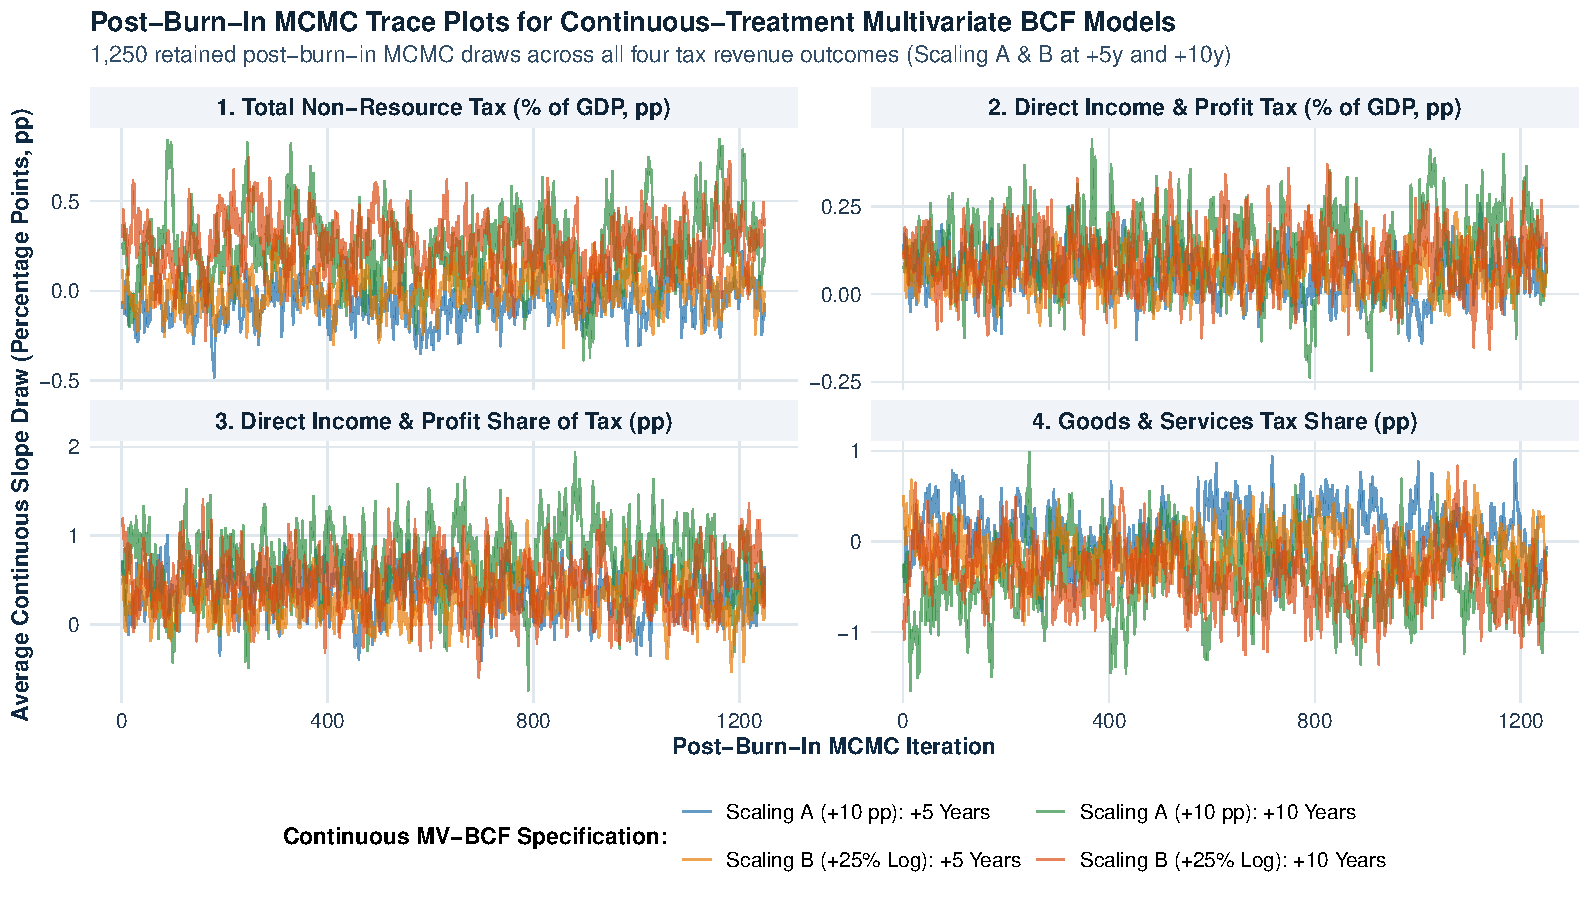
\includegraphics[width=\textwidth]{../outputs/figures/figA1_mcmc_convergence_traces.pdf}
  \caption{Post-burn-in MCMC trace plots for the Mediator-Removed Direct Fiscal Effect across all four tax outcomes from both the single-horizon \texttt{mvbcf} ($+5\text{y}$ and $+10\text{y}$) and the cumulative 10-year \texttt{lbcf} sampler.}
  \label{fig:traces}
\end{figure}

\section{Computational Environment and Energy Report}
\label{app:compute}

All data processing, C++ (\texttt{RcppArmadillo}) Gibbs sampling, and figure generation were executed on a single Apple Silicon workstation (\texttt{macOS}, R version 4.6.1, Apple Clang C++17 compiler). Table~\ref{tab:compute} reports the exact wall-clock runtime, estimated electrical energy use (assuming an average 25~W CPU package thermal design power during single-core C++ tree sampling), and estimated carbon emissions (using the Irish grid average carbon intensity of $250\text{ g CO}_2\text{e/kWh}$).

\begin{table}[ht!]
  \centering
  \caption{Computational wall-clock time, energy use, and estimated carbon footprint across the modelling pipeline.}
  \label{tab:compute}
  \small
  \setlength{\tabcolsep}{4.8pt}
  \begin{tabular}{l|l|c|c|c}
    \toprule
    \rowcolor{tabhead}
    \textbf{Pipeline Stage} & \textbf{Models Fitted} & \textbf{Time (s)} & \textbf{Energy (Wh)} & \textbf{$\text{CO}_2\text{e}$ (g)} \\
    \midrule
    \rowcolor{rowodd}
    Step 04: \texttt{mvbcf} \& Benchmarks & \co 30 four-outcome fits (2,000 iter) & 611.4 & \co 4.25 & 1.06 \\
    \rowcolor{roweven}
    Step 05: Longitudinal \texttt{lbcf} & \ce 4 two-increment fits (2,500 iter) & 204.5 & \ce 1.42 & 0.36 \\
    \midrule
    \rowcolor{tabhead}
    \textbf{Total Pipeline} & \textbf{All 34 model fits} & \textbf{815.9} & \textbf{5.67} & \textbf{1.42} \\
    \bottomrule
  \end{tabular}
\end{table}

\clearpage
\bibliographystyle{abbrvnat}
\bibliography{references}

\end{document}
